% Options for packages loaded elsewhere
\PassOptionsToPackage{unicode}{hyperref}
\PassOptionsToPackage{hyphens}{url}
%
\documentclass[
  a4paper,
]{scrbook}

\usepackage{amsmath,amssymb}
\usepackage{iftex}
\ifPDFTeX
  \usepackage[T1]{fontenc}
  \usepackage[utf8]{inputenc}
  \usepackage{textcomp} % provide euro and other symbols
\else % if luatex or xetex
  \usepackage{unicode-math}
  \defaultfontfeatures{Scale=MatchLowercase}
  \defaultfontfeatures[\rmfamily]{Ligatures=TeX,Scale=1}
\fi
\usepackage{lmodern}
\ifPDFTeX\else  
    % xetex/luatex font selection
\fi
% Use upquote if available, for straight quotes in verbatim environments
\IfFileExists{upquote.sty}{\usepackage{upquote}}{}
\IfFileExists{microtype.sty}{% use microtype if available
  \usepackage[]{microtype}
  \UseMicrotypeSet[protrusion]{basicmath} % disable protrusion for tt fonts
}{}
\makeatletter
\@ifundefined{KOMAClassName}{% if non-KOMA class
  \IfFileExists{parskip.sty}{%
    \usepackage{parskip}
  }{% else
    \setlength{\parindent}{0pt}
    \setlength{\parskip}{6pt plus 2pt minus 1pt}}
}{% if KOMA class
  \KOMAoptions{parskip=half}}
\makeatother
\usepackage{xcolor}
\setlength{\emergencystretch}{3em} % prevent overfull lines
\setcounter{secnumdepth}{5}
% Make \paragraph and \subparagraph free-standing
\makeatletter
\ifx\paragraph\undefined\else
  \let\oldparagraph\paragraph
  \renewcommand{\paragraph}{
    \@ifstar
      \xxxParagraphStar
      \xxxParagraphNoStar
  }
  \newcommand{\xxxParagraphStar}[1]{\oldparagraph*{#1}\mbox{}}
  \newcommand{\xxxParagraphNoStar}[1]{\oldparagraph{#1}\mbox{}}
\fi
\ifx\subparagraph\undefined\else
  \let\oldsubparagraph\subparagraph
  \renewcommand{\subparagraph}{
    \@ifstar
      \xxxSubParagraphStar
      \xxxSubParagraphNoStar
  }
  \newcommand{\xxxSubParagraphStar}[1]{\oldsubparagraph*{#1}\mbox{}}
  \newcommand{\xxxSubParagraphNoStar}[1]{\oldsubparagraph{#1}\mbox{}}
\fi
\makeatother

\usepackage{color}
\usepackage{fancyvrb}
\newcommand{\VerbBar}{|}
\newcommand{\VERB}{\Verb[commandchars=\\\{\}]}
\DefineVerbatimEnvironment{Highlighting}{Verbatim}{commandchars=\\\{\}}
% Add ',fontsize=\small' for more characters per line
\usepackage{framed}
\definecolor{shadecolor}{RGB}{241,243,245}
\newenvironment{Shaded}{\begin{snugshade}}{\end{snugshade}}
\newcommand{\AlertTok}[1]{\textcolor[rgb]{0.68,0.00,0.00}{#1}}
\newcommand{\AnnotationTok}[1]{\textcolor[rgb]{0.37,0.37,0.37}{#1}}
\newcommand{\AttributeTok}[1]{\textcolor[rgb]{0.40,0.45,0.13}{#1}}
\newcommand{\BaseNTok}[1]{\textcolor[rgb]{0.68,0.00,0.00}{#1}}
\newcommand{\BuiltInTok}[1]{\textcolor[rgb]{0.00,0.23,0.31}{#1}}
\newcommand{\CharTok}[1]{\textcolor[rgb]{0.13,0.47,0.30}{#1}}
\newcommand{\CommentTok}[1]{\textcolor[rgb]{0.37,0.37,0.37}{#1}}
\newcommand{\CommentVarTok}[1]{\textcolor[rgb]{0.37,0.37,0.37}{\textit{#1}}}
\newcommand{\ConstantTok}[1]{\textcolor[rgb]{0.56,0.35,0.01}{#1}}
\newcommand{\ControlFlowTok}[1]{\textcolor[rgb]{0.00,0.23,0.31}{\textbf{#1}}}
\newcommand{\DataTypeTok}[1]{\textcolor[rgb]{0.68,0.00,0.00}{#1}}
\newcommand{\DecValTok}[1]{\textcolor[rgb]{0.68,0.00,0.00}{#1}}
\newcommand{\DocumentationTok}[1]{\textcolor[rgb]{0.37,0.37,0.37}{\textit{#1}}}
\newcommand{\ErrorTok}[1]{\textcolor[rgb]{0.68,0.00,0.00}{#1}}
\newcommand{\ExtensionTok}[1]{\textcolor[rgb]{0.00,0.23,0.31}{#1}}
\newcommand{\FloatTok}[1]{\textcolor[rgb]{0.68,0.00,0.00}{#1}}
\newcommand{\FunctionTok}[1]{\textcolor[rgb]{0.28,0.35,0.67}{#1}}
\newcommand{\ImportTok}[1]{\textcolor[rgb]{0.00,0.46,0.62}{#1}}
\newcommand{\InformationTok}[1]{\textcolor[rgb]{0.37,0.37,0.37}{#1}}
\newcommand{\KeywordTok}[1]{\textcolor[rgb]{0.00,0.23,0.31}{\textbf{#1}}}
\newcommand{\NormalTok}[1]{\textcolor[rgb]{0.00,0.23,0.31}{#1}}
\newcommand{\OperatorTok}[1]{\textcolor[rgb]{0.37,0.37,0.37}{#1}}
\newcommand{\OtherTok}[1]{\textcolor[rgb]{0.00,0.23,0.31}{#1}}
\newcommand{\PreprocessorTok}[1]{\textcolor[rgb]{0.68,0.00,0.00}{#1}}
\newcommand{\RegionMarkerTok}[1]{\textcolor[rgb]{0.00,0.23,0.31}{#1}}
\newcommand{\SpecialCharTok}[1]{\textcolor[rgb]{0.37,0.37,0.37}{#1}}
\newcommand{\SpecialStringTok}[1]{\textcolor[rgb]{0.13,0.47,0.30}{#1}}
\newcommand{\StringTok}[1]{\textcolor[rgb]{0.13,0.47,0.30}{#1}}
\newcommand{\VariableTok}[1]{\textcolor[rgb]{0.07,0.07,0.07}{#1}}
\newcommand{\VerbatimStringTok}[1]{\textcolor[rgb]{0.13,0.47,0.30}{#1}}
\newcommand{\WarningTok}[1]{\textcolor[rgb]{0.37,0.37,0.37}{\textit{#1}}}

\providecommand{\tightlist}{%
  \setlength{\itemsep}{0pt}\setlength{\parskip}{0pt}}\usepackage{longtable,booktabs,array}
\usepackage{calc} % for calculating minipage widths
% Correct order of tables after \paragraph or \subparagraph
\usepackage{etoolbox}
\makeatletter
\patchcmd\longtable{\par}{\if@noskipsec\mbox{}\fi\par}{}{}
\makeatother
% Allow footnotes in longtable head/foot
\IfFileExists{footnotehyper.sty}{\usepackage{footnotehyper}}{\usepackage{footnote}}
\makesavenoteenv{longtable}
\usepackage{graphicx}
\makeatletter
\def\maxwidth{\ifdim\Gin@nat@width>\linewidth\linewidth\else\Gin@nat@width\fi}
\def\maxheight{\ifdim\Gin@nat@height>\textheight\textheight\else\Gin@nat@height\fi}
\makeatother
% Scale images if necessary, so that they will not overflow the page
% margins by default, and it is still possible to overwrite the defaults
% using explicit options in \includegraphics[width, height, ...]{}
\setkeys{Gin}{width=\maxwidth,height=\maxheight,keepaspectratio}
% Set default figure placement to htbp
\makeatletter
\def\fps@figure{htbp}
\makeatother
% definitions for citeproc citations
\NewDocumentCommand\citeproctext{}{}
\NewDocumentCommand\citeproc{mm}{%
  \begingroup\def\citeproctext{#2}\cite{#1}\endgroup}
\makeatletter
 % allow citations to break across lines
 \let\@cite@ofmt\@firstofone
 % avoid brackets around text for \cite:
 \def\@biblabel#1{}
 \def\@cite#1#2{{#1\if@tempswa , #2\fi}}
\makeatother
\newlength{\cslhangindent}
\setlength{\cslhangindent}{1.5em}
\newlength{\csllabelwidth}
\setlength{\csllabelwidth}{3em}
\newenvironment{CSLReferences}[2] % #1 hanging-indent, #2 entry-spacing
 {\begin{list}{}{%
  \setlength{\itemindent}{0pt}
  \setlength{\leftmargin}{0pt}
  \setlength{\parsep}{0pt}
  % turn on hanging indent if param 1 is 1
  \ifodd #1
   \setlength{\leftmargin}{\cslhangindent}
   \setlength{\itemindent}{-1\cslhangindent}
  \fi
  % set entry spacing
  \setlength{\itemsep}{#2\baselineskip}}}
 {\end{list}}
\usepackage{calc}
\newcommand{\CSLBlock}[1]{\hfill\break\parbox[t]{\linewidth}{\strut\ignorespaces#1\strut}}
\newcommand{\CSLLeftMargin}[1]{\parbox[t]{\csllabelwidth}{\strut#1\strut}}
\newcommand{\CSLRightInline}[1]{\parbox[t]{\linewidth - \csllabelwidth}{\strut#1\strut}}
\newcommand{\CSLIndent}[1]{\hspace{\cslhangindent}#1}

\makeatletter
\@ifpackageloaded{tcolorbox}{}{\usepackage[skins,breakable]{tcolorbox}}
\@ifpackageloaded{fontawesome5}{}{\usepackage{fontawesome5}}
\definecolor{quarto-callout-color}{HTML}{909090}
\definecolor{quarto-callout-note-color}{HTML}{0758E5}
\definecolor{quarto-callout-important-color}{HTML}{CC1914}
\definecolor{quarto-callout-warning-color}{HTML}{EB9113}
\definecolor{quarto-callout-tip-color}{HTML}{00A047}
\definecolor{quarto-callout-caution-color}{HTML}{FC5300}
\definecolor{quarto-callout-color-frame}{HTML}{acacac}
\definecolor{quarto-callout-note-color-frame}{HTML}{4582ec}
\definecolor{quarto-callout-important-color-frame}{HTML}{d9534f}
\definecolor{quarto-callout-warning-color-frame}{HTML}{f0ad4e}
\definecolor{quarto-callout-tip-color-frame}{HTML}{02b875}
\definecolor{quarto-callout-caution-color-frame}{HTML}{fd7e14}
\makeatother
\makeatletter
\@ifpackageloaded{bookmark}{}{\usepackage{bookmark}}
\makeatother
\makeatletter
\@ifpackageloaded{caption}{}{\usepackage{caption}}
\AtBeginDocument{%
\ifdefined\contentsname
  \renewcommand*\contentsname{Table of contents}
\else
  \newcommand\contentsname{Table of contents}
\fi
\ifdefined\listfigurename
  \renewcommand*\listfigurename{List of Figures}
\else
  \newcommand\listfigurename{List of Figures}
\fi
\ifdefined\listtablename
  \renewcommand*\listtablename{List of Tables}
\else
  \newcommand\listtablename{List of Tables}
\fi
\ifdefined\figurename
  \renewcommand*\figurename{Figure}
\else
  \newcommand\figurename{Figure}
\fi
\ifdefined\tablename
  \renewcommand*\tablename{Table}
\else
  \newcommand\tablename{Table}
\fi
}
\@ifpackageloaded{float}{}{\usepackage{float}}
\floatstyle{ruled}
\@ifundefined{c@chapter}{\newfloat{codelisting}{h}{lop}}{\newfloat{codelisting}{h}{lop}[chapter]}
\floatname{codelisting}{Listing}
\newcommand*\listoflistings{\listof{codelisting}{List of Listings}}
\makeatother
\makeatletter
\makeatother
\makeatletter
\@ifpackageloaded{caption}{}{\usepackage{caption}}
\@ifpackageloaded{subcaption}{}{\usepackage{subcaption}}
\makeatother

\ifLuaTeX
  \usepackage{selnolig}  % disable illegal ligatures
\fi
\usepackage{bookmark}

\IfFileExists{xurl.sty}{\usepackage{xurl}}{} % add URL line breaks if available
\urlstyle{same} % disable monospaced font for URLs
\hypersetup{
  pdftitle={INTRODUCTION TO DIGITAL MUSICOLOGY},
  pdfauthor={Fabian C. Moss},
  hidelinks,
  pdfcreator={LaTeX via pandoc}}


\title{INTRODUCTION TO DIGITAL MUSICOLOGY}
\author{Fabian C. Moss}
\date{2025-07-05}

\begin{document}
\frontmatter
\maketitle

\renewcommand*\contentsname{Table of contents}
{
\setcounter{tocdepth}{2}
\tableofcontents
}

\mainmatter
\bookmarksetup{startatroot}

\chapter*{Preface}\label{preface}
\addcontentsline{toc}{chapter}{Preface}

\markboth{Preface}{Preface}

This page contains material for the course \textbf{Introduction to
Digital Musicology}, held at Julius-Maximilians-Universität, Würzburg
(Germany) in Fall 2025.

\begin{tcolorbox}[enhanced jigsaw, breakable, title=\textcolor{quarto-callout-warning-color}{\faExclamationTriangle}\hspace{0.5em}{Warning}, bottomtitle=1mm, leftrule=.75mm, colbacktitle=quarto-callout-warning-color!10!white, toprule=.15mm, left=2mm, titlerule=0mm, colback=white, opacityback=0, rightrule=.15mm, arc=.35mm, colframe=quarto-callout-warning-color-frame, coltitle=black, bottomrule=.15mm, toptitle=1mm, opacitybacktitle=0.6]

This is work in progress.

\end{tcolorbox}

Test citation Knuth (1984).

\part{INTRODUCTION}

\chapter{What is Digital Musicology?}\label{what-is-digital-musicology}

Introduction and terminology

\begin{tcolorbox}[enhanced jigsaw, breakable, title=\textcolor{quarto-callout-note-color}{\faInfo}\hspace{0.5em}{Goal}, bottomtitle=1mm, leftrule=.75mm, colbacktitle=quarto-callout-note-color!10!white, toprule=.15mm, left=2mm, titlerule=0mm, colback=white, opacityback=0, rightrule=.15mm, arc=.35mm, colframe=quarto-callout-note-color-frame, coltitle=black, bottomrule=.15mm, toptitle=1mm, opacitybacktitle=0.6]

Understanding what ``digital musicology'' means.

\end{tcolorbox}

\begin{itemize}
\tightlist
\item
  Introduction
\item
  Overview of the field
\item
  Terminology

  \begin{itemize}
  \tightlist
  \item
    e.g.~digital vs computational; the latter in 2nd semester
  \item
    digital vs empirical vs quantiative
  \item
    how does DM relate to ``traditional'' subdivisions of musicology?
  \end{itemize}
\end{itemize}

\begin{tcolorbox}[enhanced jigsaw, breakable, title=\textcolor{quarto-callout-tip-color}{\faLightbulb}\hspace{0.5em}{\textbf{Exercise}}, bottomtitle=1mm, leftrule=.75mm, colbacktitle=quarto-callout-tip-color!10!white, toprule=.15mm, left=2mm, titlerule=0mm, colback=white, opacityback=0, rightrule=.15mm, arc=.35mm, colframe=quarto-callout-tip-color-frame, coltitle=black, bottomrule=.15mm, toptitle=1mm, opacitybacktitle=0.6]

Read.

\end{tcolorbox}

\chapter{Digital Musicology today}\label{digital-musicology-today}

\begin{tcolorbox}[enhanced jigsaw, breakable, title=\textcolor{quarto-callout-note-color}{\faInfo}\hspace{0.5em}{Goal}, bottomtitle=1mm, leftrule=.75mm, colbacktitle=quarto-callout-note-color!10!white, toprule=.15mm, left=2mm, titlerule=0mm, colback=white, opacityback=0, rightrule=.15mm, arc=.35mm, colframe=quarto-callout-note-color-frame, coltitle=black, bottomrule=.15mm, toptitle=1mm, opacitybacktitle=0.6]

Acquiring and overview of current activities in Digital Musicology.

\end{tcolorbox}

\begin{itemize}
\tightlist
\item
  Current research topics
\item
  Important institutions and people (also, e.g.~NFDI4Culture)
\item
  Central journals and conferences
\end{itemize}

\chapter{The history of Digital
Musicology}\label{the-history-of-digital-musicology}

\begin{tcolorbox}[enhanced jigsaw, breakable, title=\textcolor{quarto-callout-note-color}{\faInfo}\hspace{0.5em}{Goal}, bottomtitle=1mm, leftrule=.75mm, colbacktitle=quarto-callout-note-color!10!white, toprule=.15mm, left=2mm, titlerule=0mm, colback=white, opacityback=0, rightrule=.15mm, arc=.35mm, colframe=quarto-callout-note-color-frame, coltitle=black, bottomrule=.15mm, toptitle=1mm, opacitybacktitle=0.6]

Knowing the beginnings and the major stages of DM.

\end{tcolorbox}

\part{DATA ABOUT MUSIC}

\chapter{RISM metadata}\label{rism-metadata}

\begin{tcolorbox}[enhanced jigsaw, breakable, title=\textcolor{quarto-callout-note-color}{\faInfo}\hspace{0.5em}{Goal}, bottomtitle=1mm, leftrule=.75mm, colbacktitle=quarto-callout-note-color!10!white, toprule=.15mm, left=2mm, titlerule=0mm, colback=white, opacityback=0, rightrule=.15mm, arc=.35mm, colframe=quarto-callout-note-color-frame, coltitle=black, bottomrule=.15mm, toptitle=1mm, opacitybacktitle=0.6]

Learn what metadata are and how to search for music sources on RISM
Online.

\end{tcolorbox}

\begin{itemize}
\tightlist
\item
  What is RISM?
\item
  What is RISM Online?
\end{itemize}

\begin{tcolorbox}[enhanced jigsaw, breakable, title=\textcolor{quarto-callout-tip-color}{\faLightbulb}\hspace{0.5em}{Exercise}, bottomtitle=1mm, leftrule=.75mm, colbacktitle=quarto-callout-tip-color!10!white, toprule=.15mm, left=2mm, titlerule=0mm, colback=white, opacityback=0, rightrule=.15mm, arc=.35mm, colframe=quarto-callout-tip-color-frame, coltitle=black, bottomrule=.15mm, toptitle=1mm, opacitybacktitle=0.6]

Understand basic SPARQL and design queries via prompting.

\end{tcolorbox}

\chapter{Spotify and MusicBrainz
metadata}\label{spotify-and-musicbrainz-metadata}

\begin{tcolorbox}[enhanced jigsaw, breakable, title=\textcolor{quarto-callout-note-color}{\faInfo}\hspace{0.5em}{Goal}, bottomtitle=1mm, leftrule=.75mm, colbacktitle=quarto-callout-note-color!10!white, toprule=.15mm, left=2mm, titlerule=0mm, colback=white, opacityback=0, rightrule=.15mm, arc=.35mm, colframe=quarto-callout-note-color-frame, coltitle=black, bottomrule=.15mm, toptitle=1mm, opacitybacktitle=0.6]

Understand the kind of metadata provided by Spotify vs MusicBrainz.

\end{tcolorbox}

\chapter{Music and the streaming
industry}\label{music-and-the-streaming-industry}

\begin{tcolorbox}[enhanced jigsaw, breakable, title=\textcolor{quarto-callout-note-color}{\faInfo}\hspace{0.5em}{Goal}, bottomtitle=1mm, leftrule=.75mm, colbacktitle=quarto-callout-note-color!10!white, toprule=.15mm, left=2mm, titlerule=0mm, colback=white, opacityback=0, rightrule=.15mm, arc=.35mm, colframe=quarto-callout-note-color-frame, coltitle=black, bottomrule=.15mm, toptitle=1mm, opacitybacktitle=0.6]

Gain first insights into the music market and its workings.

\end{tcolorbox}

\begin{tcolorbox}[enhanced jigsaw, breakable, title=\textcolor{quarto-callout-tip-color}{\faLightbulb}\hspace{0.5em}{Exercise}, bottomtitle=1mm, leftrule=.75mm, colbacktitle=quarto-callout-tip-color!10!white, toprule=.15mm, left=2mm, titlerule=0mm, colback=white, opacityback=0, rightrule=.15mm, arc=.35mm, colframe=quarto-callout-tip-color-frame, coltitle=black, bottomrule=.15mm, toptitle=1mm, opacitybacktitle=0.6]

Work with sales data.

\end{tcolorbox}

\chapter{Analyzing song survival}\label{analyzing-song-survival}

In this session, we will analyze songs from the Billboard 100 charts and
trace their `course of life' in the charts.

The data was obtained from
\href{https://www.kaggle.com/datasets/dhruvildave/billboard-the-hot-100-songs}{Kaggle},
a large community website for data analysis challenges.

As before, we first import the \texttt{pandas} library for data analysis
and load the data using the \texttt{read\_csv} fundtion that takes as
its main argument the path to the data file, in our case
\texttt{charts.csv}.

\begin{Shaded}
\begin{Highlighting}[]
\ImportTok{import}\NormalTok{ pandas }\ImportTok{as}\NormalTok{ pd}
\NormalTok{df }\OperatorTok{=}\NormalTok{ pd.read\_csv(}\StringTok{"charts.csv"}\NormalTok{)}
\end{Highlighting}
\end{Shaded}

Inspecting the first 5 lines with the \texttt{.head()} method of pandas
DataFrames, we obtain an understanding of the structure of the data.

\begin{Shaded}
\begin{Highlighting}[]
\NormalTok{df.head()}
\end{Highlighting}
\end{Shaded}

\begin{longtable}[]{@{}llllllll@{}}
\toprule\noalign{}
& date & rank & song & artist & last-week & peak-rank &
weeks-on-board \\
\midrule\noalign{}
\endhead
\bottomrule\noalign{}
\endlastfoot
0 & 2021-11-06 & 1 & Easy On Me & Adele & 1.0 & 1 & 3 \\
1 & 2021-11-06 & 2 & Stay & The Kid LAROI \& Justin Bieber & 2.0 & 1 &
16 \\
2 & 2021-11-06 & 3 & Industry Baby & Lil Nas X \& Jack Harlow & 3.0 & 1
& 14 \\
3 & 2021-11-06 & 4 & Fancy Like & Walker Hayes & 4.0 & 3 & 19 \\
4 & 2021-11-06 & 5 & Bad Habits & Ed Sheeran & 5.0 & 2 & 18 \\
\end{longtable}

\textbf{Think:} What do the columns represent? Provide verbal
descriptions of their meaning and write it down.

After this general overview, we might want to achieve a slightly deeper
understanding. For instance, it is not difficult to interpret the
\texttt{date} column, but from only the first few entries, we cannot
know the temporal extend of our data.

Let's find out what the earliest and latest dates are using the
\texttt{.min()} and \texttt{.max()} methods, respectively.

\begin{Shaded}
\begin{Highlighting}[]
\NormalTok{df[}\StringTok{"date"}\NormalTok{].}\BuiltInTok{min}\NormalTok{(), df[}\StringTok{"date"}\NormalTok{].}\BuiltInTok{max}\NormalTok{()}
\end{Highlighting}
\end{Shaded}

\begin{verbatim}
('1958-08-04', '2021-11-06')
\end{verbatim}

This tells us that the data stored in \texttt{charts.csv} runs from
August 1958 to November 2021 and thus allows us to trace the movement of
songs in the Billboard charts across more than 60 years.

\begin{Shaded}
\begin{Highlighting}[]
\CommentTok{\# Top artists}
\NormalTok{df.artist.value\_counts()}
\end{Highlighting}
\end{Shaded}

\begin{verbatim}
artist
Taylor Swift                                                    1023
Elton John                                                       889
Madonna                                                          857
Drake                                                            787
Kenny Chesney                                                    769
                                                                ... 
YoungBoy Never Broke Again Featuring Sherhonda Gaulden             1
Drake Featuring Chris Brown                                        1
Kehlani Featuring Jhene Aiko                                       1
DaBaby Featuring A Boogie Wit da Hoodie & London On Da Track       1
The Shins                                                          1
Name: count, Length: 10205, dtype: int64
\end{verbatim}

\begin{Shaded}
\begin{Highlighting}[]
\CommentTok{\# Longest in charts}
\NormalTok{df.sort\_values(by}\OperatorTok{=}\StringTok{"weeks{-}on{-}board"}\NormalTok{, ascending}\OperatorTok{=}\VariableTok{True}\NormalTok{).iloc[}\DecValTok{50\_000}\NormalTok{:]}
\end{Highlighting}
\end{Shaded}

\begin{longtable}[]{@{}llllllll@{}}
\toprule\noalign{}
& date & rank & song & artist & last-week & peak-rank &
weeks-on-board \\
\midrule\noalign{}
\endhead
\bottomrule\noalign{}
\endlastfoot
213768 & 1980-11-22 & 69 & Turn And Walk Away & The Babys & 79.0 & 69 &
2 \\
106440 & 2001-06-16 & 41 & Fill Me In & Craig David & 69.0 & 41 & 2 \\
106443 & 2001-06-16 & 44 & Bootylicious & Destiny\textquotesingle s
Child & 66.0 & 44 & 2 \\
106448 & 2001-06-16 & 49 & All Or Nothing & O-Town & 60.0 & 49 & 2 \\
213674 & 1980-11-29 & 75 & My Mother\textquotesingle s Eyes & Bette
Midler & 85.0 & 75 & 2 \\
... & ... & ... & ... & ... & ... & ... & ... \\
39148 & 2014-05-10 & 49 & Radioactive & Imagine Dragons & 48.0 & 3 &
87 \\
1215 & 2021-08-14 & 16 & Blinding Lights & The Weeknd & 17.0 & 1 & 87 \\
1117 & 2021-08-21 & 18 & Blinding Lights & The Weeknd & 16.0 & 1 & 88 \\
1020 & 2021-08-28 & 21 & Blinding Lights & The Weeknd & 18.0 & 1 & 89 \\
919 & 2021-09-04 & 20 & Blinding Lights & The Weeknd & 21.0 & 1 & 90 \\
\end{longtable}

\begin{Shaded}
\begin{Highlighting}[]
\NormalTok{df[}\StringTok{"date"}\NormalTok{] }\OperatorTok{=}\NormalTok{ pd.to\_datetime(df[}\StringTok{"date"}\NormalTok{])}
\end{Highlighting}
\end{Shaded}

\begin{Shaded}
\begin{Highlighting}[]
\NormalTok{df[df.artist}\OperatorTok{==}\StringTok{"Drake"}\NormalTok{].song.value\_counts()}
\end{Highlighting}
\end{Shaded}

\begin{verbatim}
song
Hotline Bling     36
God's Plan        36
Controlla         26
Fake Love         25
Nice For What     25
                  ..
Trust Issues       1
Too Much           1
Own It             1
Tuscan Leather     1
Come Thru          1
Name: count, Length: 108, dtype: int64
\end{verbatim}

\begin{Shaded}
\begin{Highlighting}[]
\NormalTok{df[df.artist}\OperatorTok{==}\StringTok{"Elton John"}\NormalTok{].song.value\_counts()}
\end{Highlighting}
\end{Shaded}

\begin{verbatim}
song
Candle In The Wind 1997/Something About The Way You Look Tonight               42
Can You Feel The Love Tonight (From "The Lion King")                           26
I Guess That's Why They Call It The Blues                                      23
The One                                                                        22
Candle In The Wind                                                             21
Little Jeannie                                                                 21
The Last Song                                                                  20
Recover Your Soul                                                              20
Believe                                                                        20
Circle Of Life (From "The Lion King")                                          20
Blessed                                                                        20
Sad Songs (say So Much)                                                        19
I Don't Wanna Go On With You Like That                                         18
Nikita                                                                         18
Bennie And The Jets                                                            18
Mama Can't Buy You Love                                                        18
Blue Eyes                                                                      18
You Can Make History (Young Again)                                             17
Sacrifice                                                                      17
Empty Garden (Hey Hey Johnny)                                                  17
Crocodile Rock                                                                 17
Goodbye Yellow Brick Road                                                      17
I'm Still Standing                                                             16
Club At The End Of The Street                                                  16
Simple Life                                                                    16
Someday Out Of The Blue                                                        15
Don't Let The Sun Go Down On Me                                                15
Island Girl                                                                    15
Daniel                                                                         15
Rocket Man                                                                     15
Healing Hands                                                                  15
The Bitch Is Back                                                              14
Who Wears These Shoes?                                                         14
Wrap Her Up                                                                    14
Sorry Seems To Be The Hardest Word                                             14
Lucy In The Sky With Diamonds                                                  14
Your Song                                                                      14
Nobody Wins                                                                    13
A Word In Spanish                                                              13
Someone Saved My Life Tonight                                                  13
You Gotta Love Someone                                                         13
In Neon                                                                        13
Chloe                                                                          13
(Sartorial Eloquence) Don't Ya Wanna Play This Game No More?                   12
Kiss The Bride                                                                 12
Saturday Night's Alright For Fighting                                          12
Grow Some Funk Of Your Own/I Feel Like A Bullet (In The Gun Of Robert Ford)    11
Made In England                                                                10
Levon                                                                          10
Victim Of Love                                                                 10
Part-Time Love                                                                 10
Honky Cat                                                                      10
Friends                                                                         9
Heartache All Over The World                                                    8
Ego                                                                             8
Tiny Dancer                                                                     7
Bite Your Lip (Get up and dance!)                                               6
Border Song                                                                     5
Name: count, dtype: int64
\end{verbatim}

\begin{Shaded}
\begin{Highlighting}[]
\KeywordTok{def}\NormalTok{ chart\_performance(artist, song):}
\NormalTok{    data }\OperatorTok{=}\NormalTok{ df[(df[}\StringTok{"artist"}\NormalTok{] }\OperatorTok{==}\NormalTok{ artist) }\OperatorTok{\&}\NormalTok{ (df[}\StringTok{"song"}\NormalTok{] }\OperatorTok{==}\NormalTok{ song)]}
\NormalTok{    data }\OperatorTok{=}\NormalTok{ data.sort\_values(by}\OperatorTok{=}\StringTok{"date"}\NormalTok{).reset\_index(drop}\OperatorTok{=}\VariableTok{True}\NormalTok{)}
\NormalTok{    data[}\StringTok{"date\_rel"}\NormalTok{] }\OperatorTok{=}\NormalTok{ pd.to\_timedelta(data[}\StringTok{"date"}\NormalTok{] }\OperatorTok{{-}}\NormalTok{ data[}\StringTok{"date"}\NormalTok{][}\DecValTok{0}\NormalTok{]).dt.days}
    \ControlFlowTok{return}\NormalTok{ data}
\end{Highlighting}
\end{Shaded}

\begin{Shaded}
\begin{Highlighting}[]
\NormalTok{test\_cases }\OperatorTok{=}\NormalTok{ \{}
    \StringTok{"Taylor Swift"}\NormalTok{: }\StringTok{"You Belong With Me"}\NormalTok{,}
    \StringTok{"Drake"}\NormalTok{: }\StringTok{"God\textquotesingle{}s Plan"}\NormalTok{,}
    \StringTok{"Elton John"}\NormalTok{: }\StringTok{"Candle In The Wind 1997/Something About The Way You Look Tonight"}\NormalTok{,}
    \StringTok{"The Weeknd"}\NormalTok{: }\StringTok{"Blinding Lights"}\NormalTok{,}
    \StringTok{"Elvis Presley"}\NormalTok{: }\StringTok{"Please Don\textquotesingle{}t Stop Loving Me"}
\NormalTok{\}}
\end{Highlighting}
\end{Shaded}

\begin{Shaded}
\begin{Highlighting}[]
\NormalTok{taylor }\OperatorTok{=}\NormalTok{ chart\_performance(}\StringTok{"Taylor Swift"}\NormalTok{, }\StringTok{"You Belong With Me"}\NormalTok{)}
\NormalTok{drake }\OperatorTok{=}\NormalTok{ chart\_performance(}\StringTok{"Drake"}\NormalTok{, }\StringTok{"God\textquotesingle{}s Plan"}\NormalTok{)}
\NormalTok{elton }\OperatorTok{=}\NormalTok{ chart\_performance(}\StringTok{"Elton John"}\NormalTok{, }\StringTok{"Candle In The Wind 1997/Something About The Way You Look Tonight"}\NormalTok{)}
\NormalTok{weeknd }\OperatorTok{=}\NormalTok{ chart\_performance(}\StringTok{"The Weeknd"}\NormalTok{, }\StringTok{"Blinding Lights"}\NormalTok{)}
\NormalTok{elvis }\OperatorTok{=}\NormalTok{ chart\_performance(}\StringTok{"Elvis Presley"}\NormalTok{, }\StringTok{"Please Don\textquotesingle{}t Stop Loving Me"}\NormalTok{)}
\end{Highlighting}
\end{Shaded}

\begin{Shaded}
\begin{Highlighting}[]
\ImportTok{import}\NormalTok{ matplotlib.pyplot }\ImportTok{as}\NormalTok{ plt}
\ImportTok{import}\NormalTok{ matplotlib }\ImportTok{as}\NormalTok{ mpl }
\NormalTok{mpl.rcParams[}\StringTok{"savefig.format"}\NormalTok{] }\OperatorTok{=} \StringTok{"pdf"}
\end{Highlighting}
\end{Shaded}

\begin{Shaded}
\begin{Highlighting}[]
\NormalTok{\_, ax }\OperatorTok{=}\NormalTok{ plt.subplots(figsize}\OperatorTok{=}\NormalTok{(}\DecValTok{15}\NormalTok{,}\DecValTok{4}\NormalTok{))}

\ControlFlowTok{for}\NormalTok{ artist, song }\KeywordTok{in}\NormalTok{ test\_cases.items():}
\NormalTok{    data }\OperatorTok{=}\NormalTok{ chart\_performance(artist, song)}
\NormalTok{    x }\OperatorTok{=}\NormalTok{ data[}\StringTok{"date"}\NormalTok{].values}
\NormalTok{    y }\OperatorTok{=}\NormalTok{ data[}\StringTok{"rank"}\NormalTok{].values}

\NormalTok{    ax.plot(x, y, marker}\OperatorTok{=}\StringTok{"."}\NormalTok{, label}\OperatorTok{=}\SpecialStringTok{f"}\SpecialCharTok{\{}\NormalTok{song}\SpecialCharTok{\}}\SpecialStringTok{ (}\SpecialCharTok{\{}\NormalTok{artist}\SpecialCharTok{\}}\SpecialStringTok{)"}\NormalTok{)}

\NormalTok{plt.gca().invert\_yaxis()}
\NormalTok{plt.legend()}
\NormalTok{plt.show()}
\end{Highlighting}
\end{Shaded}

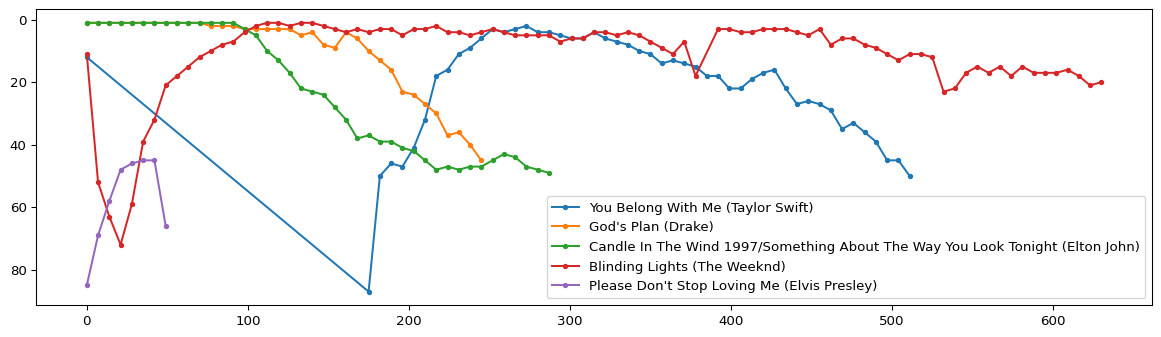
\includegraphics{data/billboard_charts_files/figure-pdf/cell-14-output-1.png}

\begin{Shaded}
\begin{Highlighting}[]
\NormalTok{\_, ax }\OperatorTok{=}\NormalTok{ plt.subplots(figsize}\OperatorTok{=}\NormalTok{(}\DecValTok{15}\NormalTok{,}\DecValTok{4}\NormalTok{))}

\ControlFlowTok{for}\NormalTok{ artist, song }\KeywordTok{in}\NormalTok{ test\_cases.items():}
\NormalTok{    data }\OperatorTok{=}\NormalTok{ chart\_performance(artist, song)}
\NormalTok{    x }\OperatorTok{=}\NormalTok{ data[}\StringTok{"date\_rel"}\NormalTok{].values}
\NormalTok{    y }\OperatorTok{=}\NormalTok{ data[}\StringTok{"rank"}\NormalTok{].values}

\NormalTok{    ax.plot(x, y, marker}\OperatorTok{=}\StringTok{"."}\NormalTok{, label}\OperatorTok{=}\SpecialStringTok{f"}\SpecialCharTok{\{}\NormalTok{song}\SpecialCharTok{\}}\SpecialStringTok{ (}\SpecialCharTok{\{}\NormalTok{artist}\SpecialCharTok{\}}\SpecialStringTok{)"}\NormalTok{)}

\NormalTok{plt.gca().invert\_yaxis()}
\NormalTok{plt.legend()}
\NormalTok{plt.show()}
\end{Highlighting}
\end{Shaded}

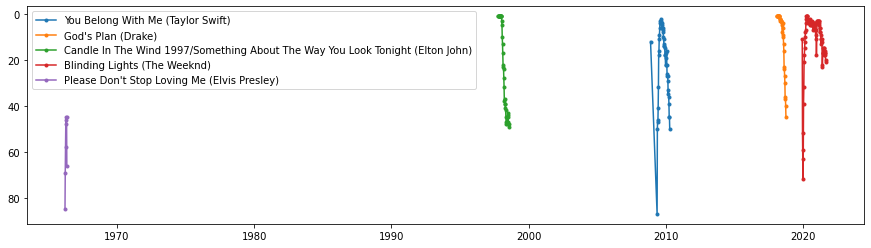
\includegraphics{data/billboard_charts_files/figure-pdf/cell-15-output-1.png}

\begin{Shaded}
\begin{Highlighting}[]
\CommentTok{\# }\AlertTok{TODO}\CommentTok{: remove lines for missing weeks (gaps in curves)}
\CommentTok{\# add two cases:}
\CommentTok{\#  {-} short duration but high peak}
\CommentTok{\#  {-} long duration but low peak}
\end{Highlighting}
\end{Shaded}

\begin{Shaded}
\begin{Highlighting}[]
\CommentTok{\# Q: can we predict a song\textquotesingle{}s survival using the features given in the data?}
\CommentTok{\# {-}{-}\textgreater{} at least introduce notion of training/test data and discuss the epistemological problem of using \textquotesingle{}all\textquotesingle{} historical }
\CommentTok{\# sources for explanation}
\end{Highlighting}
\end{Shaded}

\begin{Shaded}
\begin{Highlighting}[]
\CommentTok{\# Try other data: https://www.kaggle.com/datasets/thedevastator/billboard{-}hot{-}100{-}audio{-}features}
\end{Highlighting}
\end{Shaded}

\begin{Shaded}
\begin{Highlighting}[]
\NormalTok{df\_charts }\OperatorTok{=}\NormalTok{ pd.read\_csv(}\StringTok{"Hot Stuff.csv"}\NormalTok{, index\_col}\OperatorTok{=}\DecValTok{0}\NormalTok{)}
\NormalTok{df\_charts[}\StringTok{"WeekID"}\NormalTok{] }\OperatorTok{=}\NormalTok{ pd.to\_datetime(df\_charts[}\StringTok{"WeekID"}\NormalTok{])}
\end{Highlighting}
\end{Shaded}

\begin{Shaded}
\begin{Highlighting}[]
\NormalTok{df\_charts.head()}
\end{Highlighting}
\end{Shaded}

\begin{longtable}[]{@{}lllllllllll@{}}
\toprule\noalign{}
& url & WeekID & Week Position & Song & Performer & SongID & Instance &
Previous Week Position & Peak Position & Weeks on Chart \\
index & & & & & & & & & & \\
\midrule\noalign{}
\endhead
\bottomrule\noalign{}
\endlastfoot
0 & http://www.billboard.com/charts/hot-100/1965-0... & 1965-07-17 & 34
& Don\textquotesingle t Just Stand There & Patty Duke &
Don\textquotesingle t Just Stand TherePatty Duke & 1 & 45.0 & 34 & 4 \\
1 & http://www.billboard.com/charts/hot-100/1965-0... & 1965-07-24 & 22
& Don\textquotesingle t Just Stand There & Patty Duke &
Don\textquotesingle t Just Stand TherePatty Duke & 1 & 34.0 & 22 & 5 \\
2 & http://www.billboard.com/charts/hot-100/1965-0... & 1965-07-31 & 14
& Don\textquotesingle t Just Stand There & Patty Duke &
Don\textquotesingle t Just Stand TherePatty Duke & 1 & 22.0 & 14 & 6 \\
3 & http://www.billboard.com/charts/hot-100/1965-0... & 1965-08-07 & 10
& Don\textquotesingle t Just Stand There & Patty Duke &
Don\textquotesingle t Just Stand TherePatty Duke & 1 & 14.0 & 10 & 7 \\
4 & http://www.billboard.com/charts/hot-100/1965-0... & 1965-08-14 & 8 &
Don\textquotesingle t Just Stand There & Patty Duke &
Don\textquotesingle t Just Stand TherePatty Duke & 1 & 10.0 & 8 & 8 \\
\end{longtable}

\begin{Shaded}
\begin{Highlighting}[]
\NormalTok{df\_audio }\OperatorTok{=}\NormalTok{ pd.read\_csv(}\StringTok{"Hot 100 Audio Features.csv"}\NormalTok{, index\_col}\OperatorTok{=}\DecValTok{0}\NormalTok{)}
\end{Highlighting}
\end{Shaded}

\begin{Shaded}
\begin{Highlighting}[]
\NormalTok{df\_audio.head()}
\end{Highlighting}
\end{Shaded}

\begin{longtable}[]{@{}llllllllllllllllllllll@{}}
\toprule\noalign{}
& SongID & Performer & Song & spotify\_genre & spotify\_track\_id &
spotify\_track\_preview\_url & spotify\_track\_duration\_ms &
spotify\_track\_explicit & spotify\_track\_album & danceability & ... &
loudness & mode & speechiness & acousticness & instrumentalness &
liveness & valence & tempo & time\_signature &
spotify\_track\_popularity \\
index & & & & & & & & & & & & & & & & & & & & & \\
\midrule\noalign{}
\endhead
\bottomrule\noalign{}
\endlastfoot
0 & -twistin\textquotesingle-White Silver SandsBill
Black\textquotesingle s Combo & Bill Black\textquotesingle s Combo &
-twistin\textquotesingle-White Silver Sands & {[}{]} & NaN & NaN & NaN &
NaN & NaN & NaN & ... & NaN & NaN & NaN & NaN & NaN & NaN & NaN & NaN &
NaN & NaN \\
1 & ¿Dònde Està Santa Claus? (Where Is Santa Claus... & Augie Rios &
¿Dònde Està Santa Claus? (Where Is Santa Claus?) &
{[}\textquotesingle novelty\textquotesingle{]} & NaN & NaN & NaN & NaN &
NaN & NaN & ... & NaN & NaN & NaN & NaN & NaN & NaN & NaN & NaN & NaN &
NaN \\
2 & ......And Roses And RosesAndy Williams & Andy Williams & ......And
Roses And Roses & {[}\textquotesingle adult standards\textquotesingle,
\textquotesingle brill building pop\textquotesingle,
\textquotesingle eas... & 3tvqPPpXyIgKrm4PR9HCf0 &
https://p.scdn.co/mp3-preview/cef4883cfd1e0e53... & 166106.0 & False &
The Essential Andy Williams & 0.154 & ... & -14.063 & 1.0 & 0.0315 &
0.91100 & 0.000267 & 0.112 & 0.150 & 83.969 & 4.0 & 38.0 \\
3 & ...And Then There Were DrumsSandy Nelson & Sandy Nelson & ...And
Then There Were Drums &
{[}\textquotesingle rock-and-roll\textquotesingle,
\textquotesingle space age pop\textquotesingle, \textquotesingle surf
music\textquotesingle{]} & 1fHHq3qHU8wpRKHzhojZ4a & NaN & 172066.0 &
False & Compelling Percussion & 0.588 & ... & -17.278 & 0.0 & 0.0361 &
0.00256 & 0.745000 & 0.145 & 0.801 & 121.962 & 4.0 & 11.0 \\
4 & ...Baby One More TimeBritney Spears & Britney Spears & ...Baby One
More Time & {[}\textquotesingle dance pop\textquotesingle,
\textquotesingle pop\textquotesingle, \textquotesingle post-teen
pop\textquotesingle{]} & 3MjUtNVVq3C8Fn0MP3zhXa &
https://p.scdn.co/mp3-preview/da2134a161f1cb34... & 211066.0 & False &
...Baby One More Time (Digital Deluxe Version) & 0.759 & ... & -5.745 &
0.0 & 0.0307 & 0.20200 & 0.000131 & 0.443 & 0.907 & 92.960 & 4.0 &
77.0 \\
\end{longtable}

\begin{Shaded}
\begin{Highlighting}[]
\NormalTok{d }\OperatorTok{=}\NormalTok{ df\_charts.merge(df\_audio)}
\end{Highlighting}
\end{Shaded}

\begin{Shaded}
\begin{Highlighting}[]
\NormalTok{d.shape}
\end{Highlighting}
\end{Shaded}

\begin{verbatim}
(330208, 29)
\end{verbatim}

\begin{Shaded}
\begin{Highlighting}[]
\NormalTok{d[}\StringTok{"WeekID"}\NormalTok{] }\OperatorTok{=}\NormalTok{ pd.to\_datetime(d[}\StringTok{"WeekID"}\NormalTok{])}
\end{Highlighting}
\end{Shaded}

\begin{Shaded}
\begin{Highlighting}[]
\NormalTok{d.sample(}\DecValTok{10}\NormalTok{)}
\end{Highlighting}
\end{Shaded}

\begin{longtable}[]{@{}llllllllllllllllllllll@{}}
\toprule\noalign{}
& url & WeekID & Week Position & Song & Performer & SongID & Instance &
Previous Week Position & Peak Position & Weeks on Chart & ... & loudness
& mode & speechiness & acousticness & instrumentalness & liveness &
valence & tempo & time\_signature & spotify\_track\_popularity \\
\midrule\noalign{}
\endhead
\bottomrule\noalign{}
\endlastfoot
275610 & http://www.billboard.com/charts/hot-100/1964-0... & 1964-06-20
& 85 & My Dreams & Brenda Lee & My DreamsBrenda Lee & 1 & 96.0 & 85 & 3
& ... & NaN & NaN & NaN & NaN & NaN & NaN & NaN & NaN & NaN & NaN \\
189145 & http://www.billboard.com/charts/hot-100/2014-0... & 2014-02-08
& 97 & Radio & Darius Rucker & RadioDarius Rucker & 1 & 71.0 & 65 & 15 &
... & -6.836 & 1.0 & 0.0833 & 0.11900 & 0.000000 & 0.0606 & 0.965 &
185.939 & 4.0 & 48.0 \\
245340 & http://www.billboard.com/charts/hot-100/1969-0... & 1969-08-02
& 92 & Let\textquotesingle s Call It A Day Girl & Bobby Vee &
Let\textquotesingle s Call It A Day GirlBobby Vee & 1 & NaN & 92 & 1 &
... & NaN & NaN & NaN & NaN & NaN & NaN & NaN & NaN & NaN & NaN \\
141579 & http://www.billboard.com/charts/hot-100/2009-0... & 2009-08-08
& 3 & Knock You Down & Keri Hilson Featuring Kanye West \& Ne-Yo & Knock
You DownKeri Hilson Featuring Kanye West... & 1 & 4.0 & 3 & 18 & ... &
-4.781 & 1.0 & 0.1860 & 0.01240 & 0.000000 & 0.1770 & 0.671 & 155.171 &
4.0 & 66.0 \\
117570 & http://www.billboard.com/charts/hot-100/1960-0... & 1960-02-20
& 93 & Sleepy Lagoon & The Platters & Sleepy LagoonThe Platters & 1 &
NaN & 93 & 1 & ... & -15.519 & 1.0 & 0.0302 & 0.89400 & 0.002600 &
0.1160 & 0.541 & 68.994 & 4.0 & 33.0 \\
150750 & http://www.billboard.com/charts/hot-100/1966-0... & 1966-09-17
& 36 & Flamingo & Herb Alpert \& The Tijuana Brass & FlamingoHerb Alpert
\& The Tijuana Brass & 1 & 46.0 & 36 & 3 & ... & -9.728 & 1.0 & 0.0303 &
0.52000 & 0.765000 & 0.0745 & 0.877 & 142.111 & 4.0 & 15.0 \\
23582 & http://www.billboard.com/charts/hot-100/1985-1... & 1985-10-05 &
63 & Soul Kiss & Olivia Newton-John & Soul KissOlivia Newton-John & 1 &
NaN & 63 & 1 & ... & -15.599 & 1.0 & 0.0298 & 0.00708 & 0.001260 &
0.1130 & 0.830 & 103.222 & 4.0 & 22.0 \\
21493 & http://www.billboard.com/charts/hot-100/2003-0... & 2003-04-12 &
21 & Rock Your Body & Justin Timberlake & Rock Your BodyJustin
Timberlake & 1 & 28.0 & 21 & 4 & ... & -6.055 & 0.0 & 0.1400 & 0.20200 &
0.000234 & 0.0521 & 0.818 & 100.972 & 4.0 & 73.0 \\
71236 & http://www.billboard.com/charts/hot-100/2008-1... & 2008-12-13 &
52 & My Life & The Game Featuring Lil Wayne & My LifeThe Game Featuring
Lil Wayne & 1 & 46.0 & 21 & 17 & ... & -5.093 & 0.0 & 0.3560 & 0.07730 &
0.000000 & 0.0877 & 0.382 & 148.110 & 4.0 & 62.0 \\
208184 & http://www.billboard.com/charts/hot-100/1984-1... & 1984-12-15
& 60 & Missing You & Diana Ross & Missing YouDiana Ross & 1 & 72.0 & 60
& 3 & ... & -11.410 & 0.0 & 0.0366 & 0.65800 & 0.001160 & 0.0485 & 0.187
& 86.822 & 4.0 & 36.0 \\
\end{longtable}

\begin{Shaded}
\begin{Highlighting}[]
\CommentTok{\#\# BOOTSTRAP!}

\CommentTok{\# d = d.sample(500\_000, replace=True)}
\end{Highlighting}
\end{Shaded}

\begin{Shaded}
\begin{Highlighting}[]
\NormalTok{d.info()}
\end{Highlighting}
\end{Shaded}

\begin{verbatim}
<class 'pandas.core.frame.DataFrame'>
RangeIndex: 330208 entries, 0 to 330207
Data columns (total 29 columns):
 #   Column                     Non-Null Count   Dtype         
---  ------                     --------------   -----         
 0   url                        330208 non-null  object        
 1   WeekID                     330208 non-null  datetime64[ns]
 2   Week Position              330208 non-null  int64         
 3   Song                       330208 non-null  object        
 4   Performer                  330208 non-null  object        
 5   SongID                     330208 non-null  object        
 6   Instance                   330208 non-null  int64         
 7   Previous Week Position     298048 non-null  float64       
 8   Peak Position              330208 non-null  int64         
 9   Weeks on Chart             330208 non-null  int64         
 10  spotify_genre              315700 non-null  object        
 11  spotify_track_id           287066 non-null  object        
 12  spotify_track_preview_url  169915 non-null  object        
 13  spotify_track_duration_ms  287066 non-null  float64       
 14  spotify_track_explicit     287066 non-null  object        
 15  spotify_track_album        287004 non-null  object        
 16  danceability               286508 non-null  float64       
 17  energy                     286508 non-null  float64       
 18  key                        286508 non-null  float64       
 19  loudness                   286508 non-null  float64       
 20  mode                       286508 non-null  float64       
 21  speechiness                286508 non-null  float64       
 22  acousticness               286508 non-null  float64       
 23  instrumentalness           286508 non-null  float64       
 24  liveness                   286508 non-null  float64       
 25  valence                    286508 non-null  float64       
 26  tempo                      286508 non-null  float64       
 27  time_signature             286508 non-null  float64       
 28  spotify_track_popularity   287066 non-null  float64       
dtypes: datetime64[ns](1), float64(15), int64(4), object(9)
memory usage: 73.1+ MB
\end{verbatim}

\begin{Shaded}
\begin{Highlighting}[]
\ImportTok{from}\NormalTok{ IPython.display }\ImportTok{import}\NormalTok{ Audio, HTML}
\end{Highlighting}
\end{Shaded}

\begin{Shaded}
\begin{Highlighting}[]
\NormalTok{Audio(url}\OperatorTok{=}\NormalTok{d.loc[}\DecValTok{1000}\NormalTok{,}\StringTok{"spotify\_track\_preview\_url"}\NormalTok{])}
\end{Highlighting}
\end{Shaded}

\begin{verbatim}
<IPython.lib.display.Audio object>
\end{verbatim}

\begin{Shaded}
\begin{Highlighting}[]
\KeywordTok{def}\NormalTok{ curves(performer, song):}
\NormalTok{    data }\OperatorTok{=}\NormalTok{ d[(d.Performer }\OperatorTok{==}\NormalTok{ performer) }\OperatorTok{\&}\NormalTok{ (d.Song }\OperatorTok{==}\NormalTok{ song)].sort\_values(by}\OperatorTok{=}\StringTok{"WeekID"}\NormalTok{).reset\_index(drop}\OperatorTok{=}\VariableTok{True}\NormalTok{)}
\NormalTok{    data[}\StringTok{"date\_rel"}\NormalTok{] }\OperatorTok{=}\NormalTok{ pd.to\_timedelta(data[}\StringTok{"WeekID"}\NormalTok{] }\OperatorTok{{-}}\NormalTok{ data[}\StringTok{"WeekID"}\NormalTok{][}\DecValTok{0}\NormalTok{]).dt.days}
\NormalTok{    x }\OperatorTok{=}\NormalTok{ data[}\StringTok{"date\_rel"}\NormalTok{].values }\CommentTok{\# or date\_rel or WeekID}
\NormalTok{    y }\OperatorTok{=}\NormalTok{ data[}\StringTok{"Week Position"}\NormalTok{].values}
    \ControlFlowTok{return}\NormalTok{ x,y}
\end{Highlighting}
\end{Shaded}

\begin{Shaded}
\begin{Highlighting}[]
\NormalTok{test\_cases2 }\OperatorTok{=}\NormalTok{ \{}
    \StringTok{"Patty Duke"}\NormalTok{: }\StringTok{"Don\textquotesingle{}t Just Stand There"}\NormalTok{,}
    \StringTok{"Ace Of Base"}\NormalTok{: }\StringTok{"Don\textquotesingle{}t Turn Around"}\NormalTok{,}
    \StringTok{"Dan + Shay"}\NormalTok{: }\StringTok{"Speechless"}\NormalTok{,}
    \StringTok{"YoungBloodZ Featuring Lil Jon"}\NormalTok{: }\StringTok{"Damn!"}\NormalTok{,}
    \StringTok{"K{-}Ci \& JoJo"}\NormalTok{: }\StringTok{"All My Life"}\NormalTok{,}
    \StringTok{"Trevor Daniel"}\NormalTok{: }\StringTok{"Falling"}
\NormalTok{\}}
\end{Highlighting}
\end{Shaded}

\begin{Shaded}
\begin{Highlighting}[]
\NormalTok{\_, ax }\OperatorTok{=}\NormalTok{ plt.subplots(figsize}\OperatorTok{=}\NormalTok{(}\DecValTok{15}\NormalTok{,}\DecValTok{4}\NormalTok{))}

\ControlFlowTok{for}\NormalTok{ performer, song }\KeywordTok{in}\NormalTok{ test\_cases2.items():}
\NormalTok{    x,y }\OperatorTok{=}\NormalTok{ curves(performer, song)}
\NormalTok{    ax.plot(x, y, marker}\OperatorTok{=}\StringTok{"."}\NormalTok{, label}\OperatorTok{=}\SpecialStringTok{f"}\SpecialCharTok{\{}\NormalTok{song}\SpecialCharTok{\}}\SpecialStringTok{ (}\SpecialCharTok{\{}\NormalTok{performer}\SpecialCharTok{\}}\SpecialStringTok{)"}\NormalTok{)}

\NormalTok{plt.gca().invert\_yaxis()}
\NormalTok{plt.legend()}
\NormalTok{plt.show()}
\end{Highlighting}
\end{Shaded}

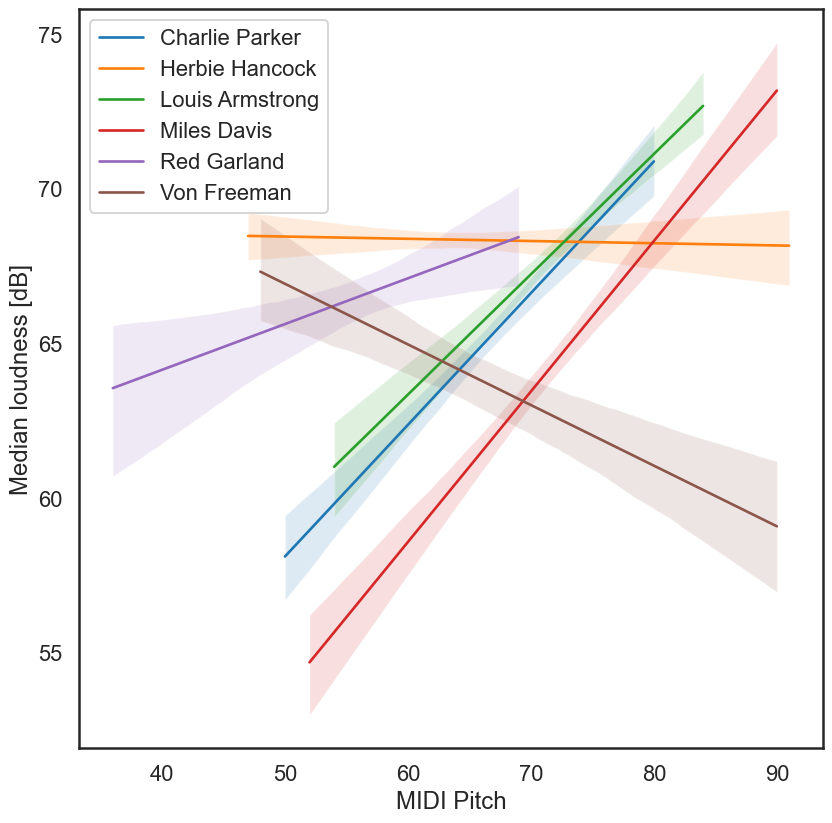
\includegraphics{data/billboard_charts_files/figure-pdf/cell-36-output-1.png}

Modeling the life of a song in the Top 100:

We assume that once a song has left the Top 100, it is impossible to
re-enter (even though that does happen, of course)

\begin{enumerate}
\def\labelenumi{\arabic{enumi}.}
\tightlist
\item
  Each song has a starting rank \(r_0\).
\item
  For each following week, there is a bernoulli dropout probability
  \(\theta\) that determines whether a song remains in the charts.
\item
\end{enumerate}

\begin{Shaded}
\begin{Highlighting}[]
\CommentTok{\# Observation: Genres tend to leave the Top 100 higher than they entered them}
\end{Highlighting}
\end{Shaded}

\begin{Shaded}
\begin{Highlighting}[]
\NormalTok{entrances }\OperatorTok{=}\NormalTok{ []}
\NormalTok{peaks }\OperatorTok{=}\NormalTok{ []}
\NormalTok{exits }\OperatorTok{=}\NormalTok{ []}

\ControlFlowTok{for}\NormalTok{ \_, group }\KeywordTok{in}\NormalTok{ d.groupby(}\StringTok{"SongID"}\NormalTok{):}
\NormalTok{    weeks }\OperatorTok{=}\NormalTok{ group.sort\_values(by}\OperatorTok{=}\StringTok{"WeekID"}\NormalTok{)[}\StringTok{"Week Position"}\NormalTok{].values}
\NormalTok{    entrances.append(weeks[}\DecValTok{0}\NormalTok{])}
\NormalTok{    peaks.append(weeks.}\BuiltInTok{min}\NormalTok{())}
\NormalTok{    exits.append(weeks[}\OperatorTok{{-}}\DecValTok{1}\NormalTok{])}
\end{Highlighting}
\end{Shaded}

\begin{Shaded}
\begin{Highlighting}[]
\ImportTok{import}\NormalTok{ numpy }\ImportTok{as}\NormalTok{ np}
\end{Highlighting}
\end{Shaded}

\begin{Shaded}
\begin{Highlighting}[]
\CommentTok{\# from matplotlib.collections import LineCollection}
\end{Highlighting}
\end{Shaded}

\begin{Shaded}
\begin{Highlighting}[]
\NormalTok{\_, ax }\OperatorTok{=}\NormalTok{ plt.subplots(figsize}\OperatorTok{=}\NormalTok{(}\DecValTok{10}\NormalTok{,}\DecValTok{4}\NormalTok{))}

\NormalTok{K }\OperatorTok{=} \BuiltInTok{len}\NormalTok{(entrances) }\OperatorTok{+} \DecValTok{1}

\ControlFlowTok{for}\NormalTok{ a, b, c }\KeywordTok{in} \BuiltInTok{zip}\NormalTok{(entrances[:K], peaks[:K], exits[:K]):}
    \ControlFlowTok{if}\NormalTok{ a }\OperatorTok{!=}\NormalTok{ b }\OperatorTok{!=}\NormalTok{ c: }\CommentTok{\# remove constants}
\NormalTok{        ax.plot([}\DecValTok{0}\NormalTok{, }\DecValTok{1}\NormalTok{, }\DecValTok{2}\NormalTok{], [a, b, c], c}\OperatorTok{=}\StringTok{"k"}\NormalTok{, lw}\OperatorTok{=}\FloatTok{.5}\NormalTok{, alpha}\OperatorTok{=}\FloatTok{.01}\NormalTok{)}

\NormalTok{plt.xlim(}\DecValTok{0}\NormalTok{,}\DecValTok{2}\NormalTok{)}
\NormalTok{plt.ylim(}\DecValTok{0}\NormalTok{,}\DecValTok{100}\NormalTok{)}
\NormalTok{plt.gca().invert\_yaxis() }\CommentTok{\# smaller is better}
\NormalTok{plt.savefig(}\StringTok{"img/rise{-}decline.png"}\NormalTok{, dpi}\OperatorTok{=}\DecValTok{600}\NormalTok{)}
\NormalTok{plt.show()}
\end{Highlighting}
\end{Shaded}

\includegraphics{data/billboard_charts_files/figure-pdf/cell-41-output-1.png}

\textbf{OBSERVATION}: At least 3 types:

\begin{itemize}
\tightlist
\item
  constants
\item
  low in, peak, low out
\item
  low in, peak, mid out
\end{itemize}

Try to disentangle what causes the difference

\part{MUSIC AS DATA}

\chapter{Audio}\label{audio}

\begin{tcolorbox}[enhanced jigsaw, breakable, title=\textcolor{quarto-callout-note-color}{\faInfo}\hspace{0.5em}{Goal}, bottomtitle=1mm, leftrule=.75mm, colbacktitle=quarto-callout-note-color!10!white, toprule=.15mm, left=2mm, titlerule=0mm, colback=white, opacityback=0, rightrule=.15mm, arc=.35mm, colframe=quarto-callout-note-color-frame, coltitle=black, bottomrule=.15mm, toptitle=1mm, opacitybacktitle=0.6]

Understand what an audio signal is and how it is represented digitally .

\end{tcolorbox}

\begin{itemize}
\tightlist
\item
  Waveform to spectrogram
\item
  Harmonics
\item
  Timbre
\item
  Audible range and volume
\item
  reading melodies from a spectrogram
\item
  digital audio: sampling
\end{itemize}

\chapter{MIDI}\label{midi}

\begin{tcolorbox}[enhanced jigsaw, breakable, title=\textcolor{quarto-callout-note-color}{\faInfo}\hspace{0.5em}{Goal}, bottomtitle=1mm, leftrule=.75mm, colbacktitle=quarto-callout-note-color!10!white, toprule=.15mm, left=2mm, titlerule=0mm, colback=white, opacityback=0, rightrule=.15mm, arc=.35mm, colframe=quarto-callout-note-color-frame, coltitle=black, bottomrule=.15mm, toptitle=1mm, opacitybacktitle=0.6]

Be able to name use cases for MIDI. Translate MIDI numbers to pitches.

\end{tcolorbox}

\chapter{MEI - header}\label{mei---header}

\begin{tcolorbox}[enhanced jigsaw, breakable, title=\textcolor{quarto-callout-note-color}{\faInfo}\hspace{0.5em}{Goal}, bottomtitle=1mm, leftrule=.75mm, colbacktitle=quarto-callout-note-color!10!white, toprule=.15mm, left=2mm, titlerule=0mm, colback=white, opacityback=0, rightrule=.15mm, arc=.35mm, colframe=quarto-callout-note-color-frame, coltitle=black, bottomrule=.15mm, toptitle=1mm, opacitybacktitle=0.6]

Understand basic XML encoding and the skeleton structure of MEI.

\end{tcolorbox}

\begin{itemize}
\tightlist
\item
  mei friend
\end{itemize}

\chapter{MEI - the body}\label{mei---the-body}

\begin{tcolorbox}[enhanced jigsaw, breakable, title=\textcolor{quarto-callout-note-color}{\faInfo}\hspace{0.5em}{Goal}, bottomtitle=1mm, leftrule=.75mm, colbacktitle=quarto-callout-note-color!10!white, toprule=.15mm, left=2mm, titlerule=0mm, colback=white, opacityback=0, rightrule=.15mm, arc=.35mm, colframe=quarto-callout-note-color-frame, coltitle=black, bottomrule=.15mm, toptitle=1mm, opacitybacktitle=0.6]

Understand the relation between CWMN and the MEI music element.

\end{tcolorbox}

\begin{itemize}
\tightlist
\item
  MuseScore export
\item
  mei friend
\end{itemize}

\part{WORKING WITH MUSIC DATA}

\chapter{Digital music analysis:
harmony}\label{digital-music-analysis-harmony}

\begin{tcolorbox}[enhanced jigsaw, breakable, title=\textcolor{quarto-callout-note-color}{\faInfo}\hspace{0.5em}{Goal}, bottomtitle=1mm, leftrule=.75mm, colbacktitle=quarto-callout-note-color!10!white, toprule=.15mm, left=2mm, titlerule=0mm, colback=white, opacityback=0, rightrule=.15mm, arc=.35mm, colframe=quarto-callout-note-color-frame, coltitle=black, bottomrule=.15mm, toptitle=1mm, opacitybacktitle=0.6]

Understand what labeling is and why labels can be useful.

\end{tcolorbox}

\begin{itemize}
\tightlist
\item
  further MuseScore practice
\item
  segmentation and labeling
\item
  Counting chords, finding cadences
\end{itemize}

\chapter{Digital music analysis:
melody}\label{digital-music-analysis-melody}

\begin{tcolorbox}[enhanced jigsaw, breakable, title=\textcolor{quarto-callout-note-color}{\faInfo}\hspace{0.5em}{Goal}, bottomtitle=1mm, leftrule=.75mm, colbacktitle=quarto-callout-note-color!10!white, toprule=.15mm, left=2mm, titlerule=0mm, colback=white, opacityback=0, rightrule=.15mm, arc=.35mm, colframe=quarto-callout-note-color-frame, coltitle=black, bottomrule=.15mm, toptitle=1mm, opacitybacktitle=0.6]

Understand how melodic pattern matching works in principle.

\end{tcolorbox}

\begin{itemize}
\tightlist
\item
  Pattern finding in melodies (Non-Western)
\end{itemize}

\chapter{Analyzing song survival}\label{analyzing-song-survival-1}

In this session, we will analyze songs from the Billboard 100 charts and
trace their `course of life' in the charts.

The data was obtained from
\href{https://www.kaggle.com/datasets/dhruvildave/billboard-the-hot-100-songs}{Kaggle},
a large community website for data analysis challenges.

As before, we first import the \texttt{pandas} library for data analysis
and load the data using the \texttt{read\_csv} fundtion that takes as
its main argument the path to the data file, in our case
\texttt{charts.csv}.

\begin{Shaded}
\begin{Highlighting}[]
\ImportTok{import}\NormalTok{ pandas }\ImportTok{as}\NormalTok{ pd}
\NormalTok{df }\OperatorTok{=}\NormalTok{ pd.read\_csv(}\StringTok{"charts.csv"}\NormalTok{)}
\end{Highlighting}
\end{Shaded}

Inspecting the first 5 lines with the \texttt{.head()} method of pandas
DataFrames, we obtain an understanding of the structure of the data.

\begin{Shaded}
\begin{Highlighting}[]
\NormalTok{df.head()}
\end{Highlighting}
\end{Shaded}

\begin{longtable}[]{@{}llllllll@{}}
\toprule\noalign{}
& date & rank & song & artist & last-week & peak-rank &
weeks-on-board \\
\midrule\noalign{}
\endhead
\bottomrule\noalign{}
\endlastfoot
0 & 2021-11-06 & 1 & Easy On Me & Adele & 1.0 & 1 & 3 \\
1 & 2021-11-06 & 2 & Stay & The Kid LAROI \& Justin Bieber & 2.0 & 1 &
16 \\
2 & 2021-11-06 & 3 & Industry Baby & Lil Nas X \& Jack Harlow & 3.0 & 1
& 14 \\
3 & 2021-11-06 & 4 & Fancy Like & Walker Hayes & 4.0 & 3 & 19 \\
4 & 2021-11-06 & 5 & Bad Habits & Ed Sheeran & 5.0 & 2 & 18 \\
\end{longtable}

\textbf{Think:} What do the columns represent? Provide verbal
descriptions of their meaning and write it down.

After this general overview, we might want to achieve a slightly deeper
understanding. For instance, it is not difficult to interpret the
\texttt{date} column, but from only the first few entries, we cannot
know the temporal extend of our data.

Let's find out what the earliest and latest dates are using the
\texttt{.min()} and \texttt{.max()} methods, respectively.

\begin{Shaded}
\begin{Highlighting}[]
\NormalTok{df[}\StringTok{"date"}\NormalTok{].}\BuiltInTok{min}\NormalTok{(), df[}\StringTok{"date"}\NormalTok{].}\BuiltInTok{max}\NormalTok{()}
\end{Highlighting}
\end{Shaded}

\begin{verbatim}
('1958-08-04', '2021-11-06')
\end{verbatim}

This tells us that the data stored in \texttt{charts.csv} runs from
August 1958 to November 2021 and thus allows us to trace the movement of
songs in the Billboard charts across more than 60 years.

\begin{Shaded}
\begin{Highlighting}[]
\CommentTok{\# Top artists}
\NormalTok{df.artist.value\_counts()}
\end{Highlighting}
\end{Shaded}

\begin{verbatim}
artist
Taylor Swift                                                    1023
Elton John                                                       889
Madonna                                                          857
Drake                                                            787
Kenny Chesney                                                    769
                                                                ... 
YoungBoy Never Broke Again Featuring Sherhonda Gaulden             1
Drake Featuring Chris Brown                                        1
Kehlani Featuring Jhene Aiko                                       1
DaBaby Featuring A Boogie Wit da Hoodie & London On Da Track       1
The Shins                                                          1
Name: count, Length: 10205, dtype: int64
\end{verbatim}

\begin{Shaded}
\begin{Highlighting}[]
\CommentTok{\# Longest in charts}
\NormalTok{df.sort\_values(by}\OperatorTok{=}\StringTok{"weeks{-}on{-}board"}\NormalTok{, ascending}\OperatorTok{=}\VariableTok{True}\NormalTok{).iloc[}\DecValTok{50\_000}\NormalTok{:]}
\end{Highlighting}
\end{Shaded}

\begin{longtable}[]{@{}llllllll@{}}
\toprule\noalign{}
& date & rank & song & artist & last-week & peak-rank &
weeks-on-board \\
\midrule\noalign{}
\endhead
\bottomrule\noalign{}
\endlastfoot
213768 & 1980-11-22 & 69 & Turn And Walk Away & The Babys & 79.0 & 69 &
2 \\
106440 & 2001-06-16 & 41 & Fill Me In & Craig David & 69.0 & 41 & 2 \\
106443 & 2001-06-16 & 44 & Bootylicious & Destiny\textquotesingle s
Child & 66.0 & 44 & 2 \\
106448 & 2001-06-16 & 49 & All Or Nothing & O-Town & 60.0 & 49 & 2 \\
213674 & 1980-11-29 & 75 & My Mother\textquotesingle s Eyes & Bette
Midler & 85.0 & 75 & 2 \\
... & ... & ... & ... & ... & ... & ... & ... \\
39148 & 2014-05-10 & 49 & Radioactive & Imagine Dragons & 48.0 & 3 &
87 \\
1215 & 2021-08-14 & 16 & Blinding Lights & The Weeknd & 17.0 & 1 & 87 \\
1117 & 2021-08-21 & 18 & Blinding Lights & The Weeknd & 16.0 & 1 & 88 \\
1020 & 2021-08-28 & 21 & Blinding Lights & The Weeknd & 18.0 & 1 & 89 \\
919 & 2021-09-04 & 20 & Blinding Lights & The Weeknd & 21.0 & 1 & 90 \\
\end{longtable}

\begin{Shaded}
\begin{Highlighting}[]
\NormalTok{df[}\StringTok{"date"}\NormalTok{] }\OperatorTok{=}\NormalTok{ pd.to\_datetime(df[}\StringTok{"date"}\NormalTok{])}
\end{Highlighting}
\end{Shaded}

\begin{Shaded}
\begin{Highlighting}[]
\NormalTok{df[df.artist}\OperatorTok{==}\StringTok{"Drake"}\NormalTok{].song.value\_counts()}
\end{Highlighting}
\end{Shaded}

\begin{verbatim}
song
Hotline Bling     36
God's Plan        36
Controlla         26
Fake Love         25
Nice For What     25
                  ..
Trust Issues       1
Too Much           1
Own It             1
Tuscan Leather     1
Come Thru          1
Name: count, Length: 108, dtype: int64
\end{verbatim}

\begin{Shaded}
\begin{Highlighting}[]
\NormalTok{df[df.artist}\OperatorTok{==}\StringTok{"Elton John"}\NormalTok{].song.value\_counts()}
\end{Highlighting}
\end{Shaded}

\begin{verbatim}
song
Candle In The Wind 1997/Something About The Way You Look Tonight               42
Can You Feel The Love Tonight (From "The Lion King")                           26
I Guess That's Why They Call It The Blues                                      23
The One                                                                        22
Candle In The Wind                                                             21
Little Jeannie                                                                 21
The Last Song                                                                  20
Recover Your Soul                                                              20
Believe                                                                        20
Circle Of Life (From "The Lion King")                                          20
Blessed                                                                        20
Sad Songs (say So Much)                                                        19
I Don't Wanna Go On With You Like That                                         18
Nikita                                                                         18
Bennie And The Jets                                                            18
Mama Can't Buy You Love                                                        18
Blue Eyes                                                                      18
You Can Make History (Young Again)                                             17
Sacrifice                                                                      17
Empty Garden (Hey Hey Johnny)                                                  17
Crocodile Rock                                                                 17
Goodbye Yellow Brick Road                                                      17
I'm Still Standing                                                             16
Club At The End Of The Street                                                  16
Simple Life                                                                    16
Someday Out Of The Blue                                                        15
Don't Let The Sun Go Down On Me                                                15
Island Girl                                                                    15
Daniel                                                                         15
Rocket Man                                                                     15
Healing Hands                                                                  15
The Bitch Is Back                                                              14
Who Wears These Shoes?                                                         14
Wrap Her Up                                                                    14
Sorry Seems To Be The Hardest Word                                             14
Lucy In The Sky With Diamonds                                                  14
Your Song                                                                      14
Nobody Wins                                                                    13
A Word In Spanish                                                              13
Someone Saved My Life Tonight                                                  13
You Gotta Love Someone                                                         13
In Neon                                                                        13
Chloe                                                                          13
(Sartorial Eloquence) Don't Ya Wanna Play This Game No More?                   12
Kiss The Bride                                                                 12
Saturday Night's Alright For Fighting                                          12
Grow Some Funk Of Your Own/I Feel Like A Bullet (In The Gun Of Robert Ford)    11
Made In England                                                                10
Levon                                                                          10
Victim Of Love                                                                 10
Part-Time Love                                                                 10
Honky Cat                                                                      10
Friends                                                                         9
Heartache All Over The World                                                    8
Ego                                                                             8
Tiny Dancer                                                                     7
Bite Your Lip (Get up and dance!)                                               6
Border Song                                                                     5
Name: count, dtype: int64
\end{verbatim}

\begin{Shaded}
\begin{Highlighting}[]
\KeywordTok{def}\NormalTok{ chart\_performance(artist, song):}
\NormalTok{    data }\OperatorTok{=}\NormalTok{ df[(df[}\StringTok{"artist"}\NormalTok{] }\OperatorTok{==}\NormalTok{ artist) }\OperatorTok{\&}\NormalTok{ (df[}\StringTok{"song"}\NormalTok{] }\OperatorTok{==}\NormalTok{ song)]}
\NormalTok{    data }\OperatorTok{=}\NormalTok{ data.sort\_values(by}\OperatorTok{=}\StringTok{"date"}\NormalTok{).reset\_index(drop}\OperatorTok{=}\VariableTok{True}\NormalTok{)}
\NormalTok{    data[}\StringTok{"date\_rel"}\NormalTok{] }\OperatorTok{=}\NormalTok{ pd.to\_timedelta(data[}\StringTok{"date"}\NormalTok{] }\OperatorTok{{-}}\NormalTok{ data[}\StringTok{"date"}\NormalTok{][}\DecValTok{0}\NormalTok{]).dt.days}
    \ControlFlowTok{return}\NormalTok{ data}
\end{Highlighting}
\end{Shaded}

\begin{Shaded}
\begin{Highlighting}[]
\NormalTok{test\_cases }\OperatorTok{=}\NormalTok{ \{}
    \StringTok{"Taylor Swift"}\NormalTok{: }\StringTok{"You Belong With Me"}\NormalTok{,}
    \StringTok{"Drake"}\NormalTok{: }\StringTok{"God\textquotesingle{}s Plan"}\NormalTok{,}
    \StringTok{"Elton John"}\NormalTok{: }\StringTok{"Candle In The Wind 1997/Something About The Way You Look Tonight"}\NormalTok{,}
    \StringTok{"The Weeknd"}\NormalTok{: }\StringTok{"Blinding Lights"}\NormalTok{,}
    \StringTok{"Elvis Presley"}\NormalTok{: }\StringTok{"Please Don\textquotesingle{}t Stop Loving Me"}
\NormalTok{\}}
\end{Highlighting}
\end{Shaded}

\begin{Shaded}
\begin{Highlighting}[]
\NormalTok{taylor }\OperatorTok{=}\NormalTok{ chart\_performance(}\StringTok{"Taylor Swift"}\NormalTok{, }\StringTok{"You Belong With Me"}\NormalTok{)}
\NormalTok{drake }\OperatorTok{=}\NormalTok{ chart\_performance(}\StringTok{"Drake"}\NormalTok{, }\StringTok{"God\textquotesingle{}s Plan"}\NormalTok{)}
\NormalTok{elton }\OperatorTok{=}\NormalTok{ chart\_performance(}\StringTok{"Elton John"}\NormalTok{, }\StringTok{"Candle In The Wind 1997/Something About The Way You Look Tonight"}\NormalTok{)}
\NormalTok{weeknd }\OperatorTok{=}\NormalTok{ chart\_performance(}\StringTok{"The Weeknd"}\NormalTok{, }\StringTok{"Blinding Lights"}\NormalTok{)}
\NormalTok{elvis }\OperatorTok{=}\NormalTok{ chart\_performance(}\StringTok{"Elvis Presley"}\NormalTok{, }\StringTok{"Please Don\textquotesingle{}t Stop Loving Me"}\NormalTok{)}
\end{Highlighting}
\end{Shaded}

\begin{Shaded}
\begin{Highlighting}[]
\ImportTok{import}\NormalTok{ matplotlib.pyplot }\ImportTok{as}\NormalTok{ plt}
\ImportTok{import}\NormalTok{ matplotlib }\ImportTok{as}\NormalTok{ mpl }
\NormalTok{mpl.rcParams[}\StringTok{"savefig.format"}\NormalTok{] }\OperatorTok{=} \StringTok{"pdf"}
\end{Highlighting}
\end{Shaded}

\begin{Shaded}
\begin{Highlighting}[]
\NormalTok{\_, ax }\OperatorTok{=}\NormalTok{ plt.subplots(figsize}\OperatorTok{=}\NormalTok{(}\DecValTok{15}\NormalTok{,}\DecValTok{4}\NormalTok{))}

\ControlFlowTok{for}\NormalTok{ artist, song }\KeywordTok{in}\NormalTok{ test\_cases.items():}
\NormalTok{    data }\OperatorTok{=}\NormalTok{ chart\_performance(artist, song)}
\NormalTok{    x }\OperatorTok{=}\NormalTok{ data[}\StringTok{"date"}\NormalTok{].values}
\NormalTok{    y }\OperatorTok{=}\NormalTok{ data[}\StringTok{"rank"}\NormalTok{].values}

\NormalTok{    ax.plot(x, y, marker}\OperatorTok{=}\StringTok{"."}\NormalTok{, label}\OperatorTok{=}\SpecialStringTok{f"}\SpecialCharTok{\{}\NormalTok{song}\SpecialCharTok{\}}\SpecialStringTok{ (}\SpecialCharTok{\{}\NormalTok{artist}\SpecialCharTok{\}}\SpecialStringTok{)"}\NormalTok{)}

\NormalTok{plt.gca().invert\_yaxis()}
\NormalTok{plt.legend()}
\NormalTok{plt.show()}
\end{Highlighting}
\end{Shaded}

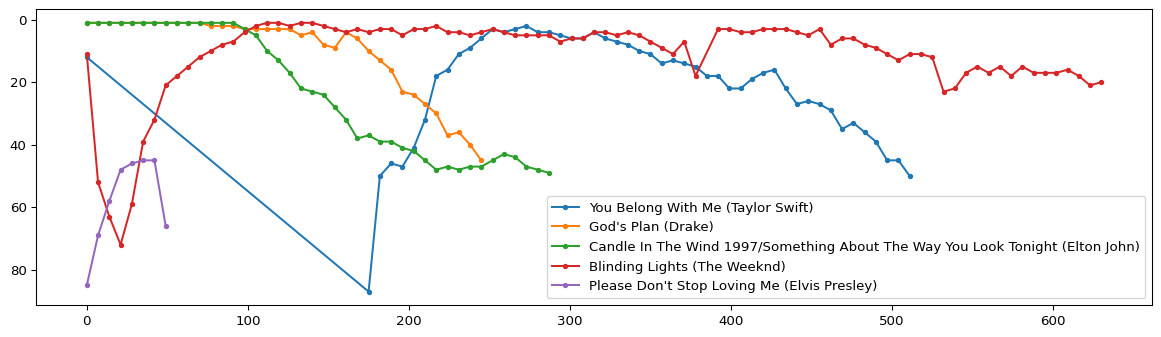
\includegraphics{data/billboard_charts_files/figure-pdf/cell-14-output-1.png}

\begin{Shaded}
\begin{Highlighting}[]
\NormalTok{\_, ax }\OperatorTok{=}\NormalTok{ plt.subplots(figsize}\OperatorTok{=}\NormalTok{(}\DecValTok{15}\NormalTok{,}\DecValTok{4}\NormalTok{))}

\ControlFlowTok{for}\NormalTok{ artist, song }\KeywordTok{in}\NormalTok{ test\_cases.items():}
\NormalTok{    data }\OperatorTok{=}\NormalTok{ chart\_performance(artist, song)}
\NormalTok{    x }\OperatorTok{=}\NormalTok{ data[}\StringTok{"date\_rel"}\NormalTok{].values}
\NormalTok{    y }\OperatorTok{=}\NormalTok{ data[}\StringTok{"rank"}\NormalTok{].values}

\NormalTok{    ax.plot(x, y, marker}\OperatorTok{=}\StringTok{"."}\NormalTok{, label}\OperatorTok{=}\SpecialStringTok{f"}\SpecialCharTok{\{}\NormalTok{song}\SpecialCharTok{\}}\SpecialStringTok{ (}\SpecialCharTok{\{}\NormalTok{artist}\SpecialCharTok{\}}\SpecialStringTok{)"}\NormalTok{)}

\NormalTok{plt.gca().invert\_yaxis()}
\NormalTok{plt.legend()}
\NormalTok{plt.show()}
\end{Highlighting}
\end{Shaded}

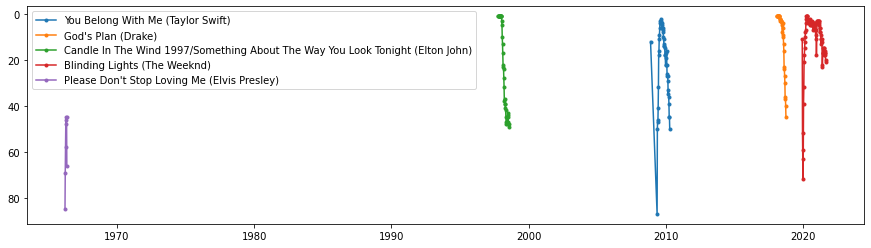
\includegraphics{data/billboard_charts_files/figure-pdf/cell-15-output-1.png}

\begin{Shaded}
\begin{Highlighting}[]
\CommentTok{\# }\AlertTok{TODO}\CommentTok{: remove lines for missing weeks (gaps in curves)}
\CommentTok{\# add two cases:}
\CommentTok{\#  {-} short duration but high peak}
\CommentTok{\#  {-} long duration but low peak}
\end{Highlighting}
\end{Shaded}

\begin{Shaded}
\begin{Highlighting}[]
\CommentTok{\# Q: can we predict a song\textquotesingle{}s survival using the features given in the data?}
\CommentTok{\# {-}{-}\textgreater{} at least introduce notion of training/test data and discuss the epistemological problem of using \textquotesingle{}all\textquotesingle{} historical }
\CommentTok{\# sources for explanation}
\end{Highlighting}
\end{Shaded}

\begin{Shaded}
\begin{Highlighting}[]
\CommentTok{\# Try other data: https://www.kaggle.com/datasets/thedevastator/billboard{-}hot{-}100{-}audio{-}features}
\end{Highlighting}
\end{Shaded}

\begin{Shaded}
\begin{Highlighting}[]
\NormalTok{df\_charts }\OperatorTok{=}\NormalTok{ pd.read\_csv(}\StringTok{"Hot Stuff.csv"}\NormalTok{, index\_col}\OperatorTok{=}\DecValTok{0}\NormalTok{)}
\NormalTok{df\_charts[}\StringTok{"WeekID"}\NormalTok{] }\OperatorTok{=}\NormalTok{ pd.to\_datetime(df\_charts[}\StringTok{"WeekID"}\NormalTok{])}
\end{Highlighting}
\end{Shaded}

\begin{Shaded}
\begin{Highlighting}[]
\NormalTok{df\_charts.head()}
\end{Highlighting}
\end{Shaded}

\begin{longtable}[]{@{}lllllllllll@{}}
\toprule\noalign{}
& url & WeekID & Week Position & Song & Performer & SongID & Instance &
Previous Week Position & Peak Position & Weeks on Chart \\
index & & & & & & & & & & \\
\midrule\noalign{}
\endhead
\bottomrule\noalign{}
\endlastfoot
0 & http://www.billboard.com/charts/hot-100/1965-0... & 1965-07-17 & 34
& Don\textquotesingle t Just Stand There & Patty Duke &
Don\textquotesingle t Just Stand TherePatty Duke & 1 & 45.0 & 34 & 4 \\
1 & http://www.billboard.com/charts/hot-100/1965-0... & 1965-07-24 & 22
& Don\textquotesingle t Just Stand There & Patty Duke &
Don\textquotesingle t Just Stand TherePatty Duke & 1 & 34.0 & 22 & 5 \\
2 & http://www.billboard.com/charts/hot-100/1965-0... & 1965-07-31 & 14
& Don\textquotesingle t Just Stand There & Patty Duke &
Don\textquotesingle t Just Stand TherePatty Duke & 1 & 22.0 & 14 & 6 \\
3 & http://www.billboard.com/charts/hot-100/1965-0... & 1965-08-07 & 10
& Don\textquotesingle t Just Stand There & Patty Duke &
Don\textquotesingle t Just Stand TherePatty Duke & 1 & 14.0 & 10 & 7 \\
4 & http://www.billboard.com/charts/hot-100/1965-0... & 1965-08-14 & 8 &
Don\textquotesingle t Just Stand There & Patty Duke &
Don\textquotesingle t Just Stand TherePatty Duke & 1 & 10.0 & 8 & 8 \\
\end{longtable}

\begin{Shaded}
\begin{Highlighting}[]
\NormalTok{df\_audio }\OperatorTok{=}\NormalTok{ pd.read\_csv(}\StringTok{"Hot 100 Audio Features.csv"}\NormalTok{, index\_col}\OperatorTok{=}\DecValTok{0}\NormalTok{)}
\end{Highlighting}
\end{Shaded}

\begin{Shaded}
\begin{Highlighting}[]
\NormalTok{df\_audio.head()}
\end{Highlighting}
\end{Shaded}

\begin{longtable}[]{@{}llllllllllllllllllllll@{}}
\toprule\noalign{}
& SongID & Performer & Song & spotify\_genre & spotify\_track\_id &
spotify\_track\_preview\_url & spotify\_track\_duration\_ms &
spotify\_track\_explicit & spotify\_track\_album & danceability & ... &
loudness & mode & speechiness & acousticness & instrumentalness &
liveness & valence & tempo & time\_signature &
spotify\_track\_popularity \\
index & & & & & & & & & & & & & & & & & & & & & \\
\midrule\noalign{}
\endhead
\bottomrule\noalign{}
\endlastfoot
0 & -twistin\textquotesingle-White Silver SandsBill
Black\textquotesingle s Combo & Bill Black\textquotesingle s Combo &
-twistin\textquotesingle-White Silver Sands & {[}{]} & NaN & NaN & NaN &
NaN & NaN & NaN & ... & NaN & NaN & NaN & NaN & NaN & NaN & NaN & NaN &
NaN & NaN \\
1 & ¿Dònde Està Santa Claus? (Where Is Santa Claus... & Augie Rios &
¿Dònde Està Santa Claus? (Where Is Santa Claus?) &
{[}\textquotesingle novelty\textquotesingle{]} & NaN & NaN & NaN & NaN &
NaN & NaN & ... & NaN & NaN & NaN & NaN & NaN & NaN & NaN & NaN & NaN &
NaN \\
2 & ......And Roses And RosesAndy Williams & Andy Williams & ......And
Roses And Roses & {[}\textquotesingle adult standards\textquotesingle,
\textquotesingle brill building pop\textquotesingle,
\textquotesingle eas... & 3tvqPPpXyIgKrm4PR9HCf0 &
https://p.scdn.co/mp3-preview/cef4883cfd1e0e53... & 166106.0 & False &
The Essential Andy Williams & 0.154 & ... & -14.063 & 1.0 & 0.0315 &
0.91100 & 0.000267 & 0.112 & 0.150 & 83.969 & 4.0 & 38.0 \\
3 & ...And Then There Were DrumsSandy Nelson & Sandy Nelson & ...And
Then There Were Drums &
{[}\textquotesingle rock-and-roll\textquotesingle,
\textquotesingle space age pop\textquotesingle, \textquotesingle surf
music\textquotesingle{]} & 1fHHq3qHU8wpRKHzhojZ4a & NaN & 172066.0 &
False & Compelling Percussion & 0.588 & ... & -17.278 & 0.0 & 0.0361 &
0.00256 & 0.745000 & 0.145 & 0.801 & 121.962 & 4.0 & 11.0 \\
4 & ...Baby One More TimeBritney Spears & Britney Spears & ...Baby One
More Time & {[}\textquotesingle dance pop\textquotesingle,
\textquotesingle pop\textquotesingle, \textquotesingle post-teen
pop\textquotesingle{]} & 3MjUtNVVq3C8Fn0MP3zhXa &
https://p.scdn.co/mp3-preview/da2134a161f1cb34... & 211066.0 & False &
...Baby One More Time (Digital Deluxe Version) & 0.759 & ... & -5.745 &
0.0 & 0.0307 & 0.20200 & 0.000131 & 0.443 & 0.907 & 92.960 & 4.0 &
77.0 \\
\end{longtable}

\begin{Shaded}
\begin{Highlighting}[]
\NormalTok{d }\OperatorTok{=}\NormalTok{ df\_charts.merge(df\_audio)}
\end{Highlighting}
\end{Shaded}

\begin{Shaded}
\begin{Highlighting}[]
\NormalTok{d.shape}
\end{Highlighting}
\end{Shaded}

\begin{verbatim}
(330208, 29)
\end{verbatim}

\begin{Shaded}
\begin{Highlighting}[]
\NormalTok{d[}\StringTok{"WeekID"}\NormalTok{] }\OperatorTok{=}\NormalTok{ pd.to\_datetime(d[}\StringTok{"WeekID"}\NormalTok{])}
\end{Highlighting}
\end{Shaded}

\begin{Shaded}
\begin{Highlighting}[]
\NormalTok{d.sample(}\DecValTok{10}\NormalTok{)}
\end{Highlighting}
\end{Shaded}

\begin{longtable}[]{@{}llllllllllllllllllllll@{}}
\toprule\noalign{}
& url & WeekID & Week Position & Song & Performer & SongID & Instance &
Previous Week Position & Peak Position & Weeks on Chart & ... & loudness
& mode & speechiness & acousticness & instrumentalness & liveness &
valence & tempo & time\_signature & spotify\_track\_popularity \\
\midrule\noalign{}
\endhead
\bottomrule\noalign{}
\endlastfoot
275610 & http://www.billboard.com/charts/hot-100/1964-0... & 1964-06-20
& 85 & My Dreams & Brenda Lee & My DreamsBrenda Lee & 1 & 96.0 & 85 & 3
& ... & NaN & NaN & NaN & NaN & NaN & NaN & NaN & NaN & NaN & NaN \\
189145 & http://www.billboard.com/charts/hot-100/2014-0... & 2014-02-08
& 97 & Radio & Darius Rucker & RadioDarius Rucker & 1 & 71.0 & 65 & 15 &
... & -6.836 & 1.0 & 0.0833 & 0.11900 & 0.000000 & 0.0606 & 0.965 &
185.939 & 4.0 & 48.0 \\
245340 & http://www.billboard.com/charts/hot-100/1969-0... & 1969-08-02
& 92 & Let\textquotesingle s Call It A Day Girl & Bobby Vee &
Let\textquotesingle s Call It A Day GirlBobby Vee & 1 & NaN & 92 & 1 &
... & NaN & NaN & NaN & NaN & NaN & NaN & NaN & NaN & NaN & NaN \\
141579 & http://www.billboard.com/charts/hot-100/2009-0... & 2009-08-08
& 3 & Knock You Down & Keri Hilson Featuring Kanye West \& Ne-Yo & Knock
You DownKeri Hilson Featuring Kanye West... & 1 & 4.0 & 3 & 18 & ... &
-4.781 & 1.0 & 0.1860 & 0.01240 & 0.000000 & 0.1770 & 0.671 & 155.171 &
4.0 & 66.0 \\
117570 & http://www.billboard.com/charts/hot-100/1960-0... & 1960-02-20
& 93 & Sleepy Lagoon & The Platters & Sleepy LagoonThe Platters & 1 &
NaN & 93 & 1 & ... & -15.519 & 1.0 & 0.0302 & 0.89400 & 0.002600 &
0.1160 & 0.541 & 68.994 & 4.0 & 33.0 \\
150750 & http://www.billboard.com/charts/hot-100/1966-0... & 1966-09-17
& 36 & Flamingo & Herb Alpert \& The Tijuana Brass & FlamingoHerb Alpert
\& The Tijuana Brass & 1 & 46.0 & 36 & 3 & ... & -9.728 & 1.0 & 0.0303 &
0.52000 & 0.765000 & 0.0745 & 0.877 & 142.111 & 4.0 & 15.0 \\
23582 & http://www.billboard.com/charts/hot-100/1985-1... & 1985-10-05 &
63 & Soul Kiss & Olivia Newton-John & Soul KissOlivia Newton-John & 1 &
NaN & 63 & 1 & ... & -15.599 & 1.0 & 0.0298 & 0.00708 & 0.001260 &
0.1130 & 0.830 & 103.222 & 4.0 & 22.0 \\
21493 & http://www.billboard.com/charts/hot-100/2003-0... & 2003-04-12 &
21 & Rock Your Body & Justin Timberlake & Rock Your BodyJustin
Timberlake & 1 & 28.0 & 21 & 4 & ... & -6.055 & 0.0 & 0.1400 & 0.20200 &
0.000234 & 0.0521 & 0.818 & 100.972 & 4.0 & 73.0 \\
71236 & http://www.billboard.com/charts/hot-100/2008-1... & 2008-12-13 &
52 & My Life & The Game Featuring Lil Wayne & My LifeThe Game Featuring
Lil Wayne & 1 & 46.0 & 21 & 17 & ... & -5.093 & 0.0 & 0.3560 & 0.07730 &
0.000000 & 0.0877 & 0.382 & 148.110 & 4.0 & 62.0 \\
208184 & http://www.billboard.com/charts/hot-100/1984-1... & 1984-12-15
& 60 & Missing You & Diana Ross & Missing YouDiana Ross & 1 & 72.0 & 60
& 3 & ... & -11.410 & 0.0 & 0.0366 & 0.65800 & 0.001160 & 0.0485 & 0.187
& 86.822 & 4.0 & 36.0 \\
\end{longtable}

\begin{Shaded}
\begin{Highlighting}[]
\CommentTok{\#\# BOOTSTRAP!}

\CommentTok{\# d = d.sample(500\_000, replace=True)}
\end{Highlighting}
\end{Shaded}

\begin{Shaded}
\begin{Highlighting}[]
\NormalTok{d.info()}
\end{Highlighting}
\end{Shaded}

\begin{verbatim}
<class 'pandas.core.frame.DataFrame'>
RangeIndex: 330208 entries, 0 to 330207
Data columns (total 29 columns):
 #   Column                     Non-Null Count   Dtype         
---  ------                     --------------   -----         
 0   url                        330208 non-null  object        
 1   WeekID                     330208 non-null  datetime64[ns]
 2   Week Position              330208 non-null  int64         
 3   Song                       330208 non-null  object        
 4   Performer                  330208 non-null  object        
 5   SongID                     330208 non-null  object        
 6   Instance                   330208 non-null  int64         
 7   Previous Week Position     298048 non-null  float64       
 8   Peak Position              330208 non-null  int64         
 9   Weeks on Chart             330208 non-null  int64         
 10  spotify_genre              315700 non-null  object        
 11  spotify_track_id           287066 non-null  object        
 12  spotify_track_preview_url  169915 non-null  object        
 13  spotify_track_duration_ms  287066 non-null  float64       
 14  spotify_track_explicit     287066 non-null  object        
 15  spotify_track_album        287004 non-null  object        
 16  danceability               286508 non-null  float64       
 17  energy                     286508 non-null  float64       
 18  key                        286508 non-null  float64       
 19  loudness                   286508 non-null  float64       
 20  mode                       286508 non-null  float64       
 21  speechiness                286508 non-null  float64       
 22  acousticness               286508 non-null  float64       
 23  instrumentalness           286508 non-null  float64       
 24  liveness                   286508 non-null  float64       
 25  valence                    286508 non-null  float64       
 26  tempo                      286508 non-null  float64       
 27  time_signature             286508 non-null  float64       
 28  spotify_track_popularity   287066 non-null  float64       
dtypes: datetime64[ns](1), float64(15), int64(4), object(9)
memory usage: 73.1+ MB
\end{verbatim}

\begin{Shaded}
\begin{Highlighting}[]
\ImportTok{from}\NormalTok{ IPython.display }\ImportTok{import}\NormalTok{ Audio, HTML}
\end{Highlighting}
\end{Shaded}

\begin{Shaded}
\begin{Highlighting}[]
\NormalTok{Audio(url}\OperatorTok{=}\NormalTok{d.loc[}\DecValTok{1000}\NormalTok{,}\StringTok{"spotify\_track\_preview\_url"}\NormalTok{])}
\end{Highlighting}
\end{Shaded}

\begin{verbatim}
<IPython.lib.display.Audio object>
\end{verbatim}

\begin{Shaded}
\begin{Highlighting}[]
\KeywordTok{def}\NormalTok{ curves(performer, song):}
\NormalTok{    data }\OperatorTok{=}\NormalTok{ d[(d.Performer }\OperatorTok{==}\NormalTok{ performer) }\OperatorTok{\&}\NormalTok{ (d.Song }\OperatorTok{==}\NormalTok{ song)].sort\_values(by}\OperatorTok{=}\StringTok{"WeekID"}\NormalTok{).reset\_index(drop}\OperatorTok{=}\VariableTok{True}\NormalTok{)}
\NormalTok{    data[}\StringTok{"date\_rel"}\NormalTok{] }\OperatorTok{=}\NormalTok{ pd.to\_timedelta(data[}\StringTok{"WeekID"}\NormalTok{] }\OperatorTok{{-}}\NormalTok{ data[}\StringTok{"WeekID"}\NormalTok{][}\DecValTok{0}\NormalTok{]).dt.days}
\NormalTok{    x }\OperatorTok{=}\NormalTok{ data[}\StringTok{"date\_rel"}\NormalTok{].values }\CommentTok{\# or date\_rel or WeekID}
\NormalTok{    y }\OperatorTok{=}\NormalTok{ data[}\StringTok{"Week Position"}\NormalTok{].values}
    \ControlFlowTok{return}\NormalTok{ x,y}
\end{Highlighting}
\end{Shaded}

\begin{Shaded}
\begin{Highlighting}[]
\NormalTok{test\_cases2 }\OperatorTok{=}\NormalTok{ \{}
    \StringTok{"Patty Duke"}\NormalTok{: }\StringTok{"Don\textquotesingle{}t Just Stand There"}\NormalTok{,}
    \StringTok{"Ace Of Base"}\NormalTok{: }\StringTok{"Don\textquotesingle{}t Turn Around"}\NormalTok{,}
    \StringTok{"Dan + Shay"}\NormalTok{: }\StringTok{"Speechless"}\NormalTok{,}
    \StringTok{"YoungBloodZ Featuring Lil Jon"}\NormalTok{: }\StringTok{"Damn!"}\NormalTok{,}
    \StringTok{"K{-}Ci \& JoJo"}\NormalTok{: }\StringTok{"All My Life"}\NormalTok{,}
    \StringTok{"Trevor Daniel"}\NormalTok{: }\StringTok{"Falling"}
\NormalTok{\}}
\end{Highlighting}
\end{Shaded}

\begin{Shaded}
\begin{Highlighting}[]
\NormalTok{\_, ax }\OperatorTok{=}\NormalTok{ plt.subplots(figsize}\OperatorTok{=}\NormalTok{(}\DecValTok{15}\NormalTok{,}\DecValTok{4}\NormalTok{))}

\ControlFlowTok{for}\NormalTok{ performer, song }\KeywordTok{in}\NormalTok{ test\_cases2.items():}
\NormalTok{    x,y }\OperatorTok{=}\NormalTok{ curves(performer, song)}
\NormalTok{    ax.plot(x, y, marker}\OperatorTok{=}\StringTok{"."}\NormalTok{, label}\OperatorTok{=}\SpecialStringTok{f"}\SpecialCharTok{\{}\NormalTok{song}\SpecialCharTok{\}}\SpecialStringTok{ (}\SpecialCharTok{\{}\NormalTok{performer}\SpecialCharTok{\}}\SpecialStringTok{)"}\NormalTok{)}

\NormalTok{plt.gca().invert\_yaxis()}
\NormalTok{plt.legend()}
\NormalTok{plt.show()}
\end{Highlighting}
\end{Shaded}

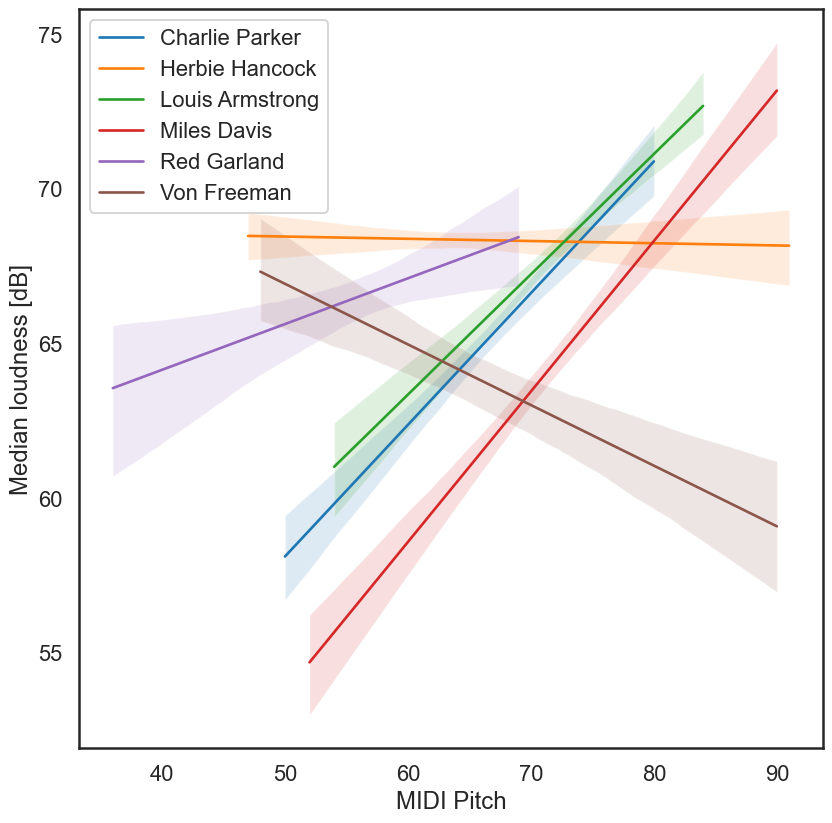
\includegraphics{data/billboard_charts_files/figure-pdf/cell-36-output-1.png}

Modeling the life of a song in the Top 100:

We assume that once a song has left the Top 100, it is impossible to
re-enter (even though that does happen, of course)

\begin{enumerate}
\def\labelenumi{\arabic{enumi}.}
\tightlist
\item
  Each song has a starting rank \(r_0\).
\item
  For each following week, there is a bernoulli dropout probability
  \(\theta\) that determines whether a song remains in the charts.
\item
\end{enumerate}

\begin{Shaded}
\begin{Highlighting}[]
\CommentTok{\# Observation: Genres tend to leave the Top 100 higher than they entered them}
\end{Highlighting}
\end{Shaded}

\begin{Shaded}
\begin{Highlighting}[]
\NormalTok{entrances }\OperatorTok{=}\NormalTok{ []}
\NormalTok{peaks }\OperatorTok{=}\NormalTok{ []}
\NormalTok{exits }\OperatorTok{=}\NormalTok{ []}

\ControlFlowTok{for}\NormalTok{ \_, group }\KeywordTok{in}\NormalTok{ d.groupby(}\StringTok{"SongID"}\NormalTok{):}
\NormalTok{    weeks }\OperatorTok{=}\NormalTok{ group.sort\_values(by}\OperatorTok{=}\StringTok{"WeekID"}\NormalTok{)[}\StringTok{"Week Position"}\NormalTok{].values}
\NormalTok{    entrances.append(weeks[}\DecValTok{0}\NormalTok{])}
\NormalTok{    peaks.append(weeks.}\BuiltInTok{min}\NormalTok{())}
\NormalTok{    exits.append(weeks[}\OperatorTok{{-}}\DecValTok{1}\NormalTok{])}
\end{Highlighting}
\end{Shaded}

\begin{Shaded}
\begin{Highlighting}[]
\ImportTok{import}\NormalTok{ numpy }\ImportTok{as}\NormalTok{ np}
\end{Highlighting}
\end{Shaded}

\begin{Shaded}
\begin{Highlighting}[]
\CommentTok{\# from matplotlib.collections import LineCollection}
\end{Highlighting}
\end{Shaded}

\begin{Shaded}
\begin{Highlighting}[]
\NormalTok{\_, ax }\OperatorTok{=}\NormalTok{ plt.subplots(figsize}\OperatorTok{=}\NormalTok{(}\DecValTok{10}\NormalTok{,}\DecValTok{4}\NormalTok{))}

\NormalTok{K }\OperatorTok{=} \BuiltInTok{len}\NormalTok{(entrances) }\OperatorTok{+} \DecValTok{1}

\ControlFlowTok{for}\NormalTok{ a, b, c }\KeywordTok{in} \BuiltInTok{zip}\NormalTok{(entrances[:K], peaks[:K], exits[:K]):}
    \ControlFlowTok{if}\NormalTok{ a }\OperatorTok{!=}\NormalTok{ b }\OperatorTok{!=}\NormalTok{ c: }\CommentTok{\# remove constants}
\NormalTok{        ax.plot([}\DecValTok{0}\NormalTok{, }\DecValTok{1}\NormalTok{, }\DecValTok{2}\NormalTok{], [a, b, c], c}\OperatorTok{=}\StringTok{"k"}\NormalTok{, lw}\OperatorTok{=}\FloatTok{.5}\NormalTok{, alpha}\OperatorTok{=}\FloatTok{.01}\NormalTok{)}

\NormalTok{plt.xlim(}\DecValTok{0}\NormalTok{,}\DecValTok{2}\NormalTok{)}
\NormalTok{plt.ylim(}\DecValTok{0}\NormalTok{,}\DecValTok{100}\NormalTok{)}
\NormalTok{plt.gca().invert\_yaxis() }\CommentTok{\# smaller is better}
\NormalTok{plt.savefig(}\StringTok{"img/rise{-}decline.png"}\NormalTok{, dpi}\OperatorTok{=}\DecValTok{600}\NormalTok{)}
\NormalTok{plt.show()}
\end{Highlighting}
\end{Shaded}

\includegraphics{data/billboard_charts_files/figure-pdf/cell-41-output-1.png}

\textbf{OBSERVATION}: At least 3 types:

\begin{itemize}
\tightlist
\item
  constants
\item
  low in, peak, low out
\item
  low in, peak, mid out
\end{itemize}

Try to disentangle what causes the difference

\part{CRITICAL DIGITAL MUSICOLOGY}

\chapter{Copyright}\label{copyright}

\begin{tcolorbox}[enhanced jigsaw, breakable, title=\textcolor{quarto-callout-note-color}{\faInfo}\hspace{0.5em}{Goal}, bottomtitle=1mm, leftrule=.75mm, colbacktitle=quarto-callout-note-color!10!white, toprule=.15mm, left=2mm, titlerule=0mm, colback=white, opacityback=0, rightrule=.15mm, arc=.35mm, colframe=quarto-callout-note-color-frame, coltitle=black, bottomrule=.15mm, toptitle=1mm, opacitybacktitle=0.6]

Know a few famous copyright infringement cases and why data analysis is
important here.

\end{tcolorbox}

\begin{itemize}
\tightlist
\item
  Plagiarism cases and copyright
\end{itemize}

\chapter{Representation and
representativeness}\label{representation-and-representativeness}

\begin{tcolorbox}[enhanced jigsaw, breakable, title=\textcolor{quarto-callout-note-color}{\faInfo}\hspace{0.5em}{Goal}, bottomtitle=1mm, leftrule=.75mm, colbacktitle=quarto-callout-note-color!10!white, toprule=.15mm, left=2mm, titlerule=0mm, colback=white, opacityback=0, rightrule=.15mm, arc=.35mm, colframe=quarto-callout-note-color-frame, coltitle=black, bottomrule=.15mm, toptitle=1mm, opacitybacktitle=0.6]

Understand the difference between representativeness and representation.
Obtain a critical understanding of biases relevant for data selection.

\end{tcolorbox}

\begin{itemize}
\tightlist
\item
  Representation and the canon
\item
  Representing means modeling means abstraction (what is ``music'' in
  ``music encoding''?)
\item
  biases: how to recognize them, how to deal with them, and when biases
  are a good thing.
\item
  FAIR and CARE
\end{itemize}

\chapter{Discussion}\label{discussion}

\begin{tcolorbox}[enhanced jigsaw, breakable, title=\textcolor{quarto-callout-note-color}{\faInfo}\hspace{0.5em}{Goal}, bottomtitle=1mm, leftrule=.75mm, colbacktitle=quarto-callout-note-color!10!white, toprule=.15mm, left=2mm, titlerule=0mm, colback=white, opacityback=0, rightrule=.15mm, arc=.35mm, colframe=quarto-callout-note-color-frame, coltitle=black, bottomrule=.15mm, toptitle=1mm, opacitybacktitle=0.6]

\end{tcolorbox}

\bookmarksetup{startatroot}

\chapter*{References}\label{references}
\addcontentsline{toc}{chapter}{References}

\markboth{References}{References}

\phantomsection\label{refs}
\begin{CSLReferences}{1}{0}
\bibitem[\citeproctext]{ref-knuth84}
Knuth, Donald E. 1984. {``Literate Programming.''} \emph{Comput. J.} 27
(2): 97--111. \url{https://doi.org/10.1093/comjnl/27.2.97}.

\end{CSLReferences}


\backmatter


\end{document}
